\chapter{Signal Efficiency}
\label{chap:eff}

A signal efficiency of finding displaced dilepton vertex is defined by the ratio of the number of events passing the signal selection (Chapter~\ref{chap:signal_selection}) to the total number of events processed. The signal efficiency can be written as Eq.~\ref{eq:OverallEff}. 

\begin{equation}
\label{eq:OverallEff}
\varepsilon_{\mathrm{overall}} = \varepsilon_{\mathrm{filter}} \cdot \varepsilon_{\mathrm{trigger}} \cdot 
                     (\varepsilon_{\mathrm{tracking}} \cdot \varepsilon_{\mathrm{lepton}})^2 \cdot
                     (\varepsilon_{\mathrm{vertexTrack}})^2 \cdot
                     \varepsilon_{\mathrm{vertexFit}}.
\end{equation}

$\varepsilon_{\mathrm{filter}}$ and $\varepsilon_{\mathrm{trigger}}$ together represent the efficiency of \texttt{RPVLL} filter, the ratio of the events passing \texttt{RPVLL} filter to the total events processed. \texttt{RPVLL} filter has the trigger filter as one of its requirements, and because it is desirable to study the trigger efficiency independently from the filter efficiency, \texttt{RPVLL} filter efficiency is factorized into the filter efficiency and the trigger efficiency. $\varepsilon_{\mathrm{tracking}}$ represents the efficiency to reconstruct ID tracks from signal particles, and $\varepsilon_{\mathrm{lepton}}$ represents the efficiency to reconstruct and identify the signal particles as leptons using ID tracks, energy deposite in calorimeters, and MS tracks. $\varepsilon_{\mathrm{vertexTrack}}$ represents the efficiency for the reconstructed signal leptons to be selected for secondary vertex reconstruction, and $\varepsilon_{\mathrm{vertexFit}}$ represents the efficiency to reconstruct a displaced vertex using two signal leptons and pass the vertex selection.
%Therefore, $\varepsilon_{\mathrm{filter}}$ is defined by the fraction of events passing \texttt{RPVLL} filter requirements without the trigger filter, and $\varepsilon_{\mathrm{trigger}}$ is defined by the fraction of events passing one of the HLTs used in this search.

In order to understand the source of signal efficiency loss, the trigger efficiency is studied in Section~\ref{sec:trigger_efficiency}, and the tracking and lepton identification efficiencies are studied in Section~\ref{sec:tracking_efficiency}. In Section~\ref{sec:combined_reco_efficiency}, the overall reconstruction efficiency, also referred as signal efficiency, of the $Z'$ signal model after the full analysis selection is presented. 

\section{Trigger efficiency}
\label{sec:trigger_efficiency}
The trigger efficiency is defined as the ratio of the events passing one of the triggers used in this analysis to the total events processed. In this analysis, three triggers listed on Table~\ref{table:triggers} are used to select the events with displaced dilepton vertex candidates. The single muon trigger is sensitive to the events with a \mumu or \emu vertex. The di-photon trigger is mainly used select the events with an \ee vertex, but a small number of events with an \emu vertex pass this trigger. The single photon trigger is sensitive to the events with \ee or \emu vertex, but its efficiency is relatively low in comparison with the other two triggers.

To illustrate the impact of the trigger efficiencies on the signal samples, the efficiency of each trigger and the combined trigger efficiency is shown in Figure~\ref{fig:m_trig_eff_allchannel} using the signal MC samples of $Z'$ decaying to all three channels at $m = $ 250 GeV and $c\tau=$ 250 mm. The sample with \ee channel shows the highest combined trigger efficiency due to the high efficiency in di-photon trigger, and the sample with \emu channel shows the reduced combined trigger efficiency because \emu vertices have only one track that can satisfy either the single muon or photon trigger.

\begin{figure}[!htb]
	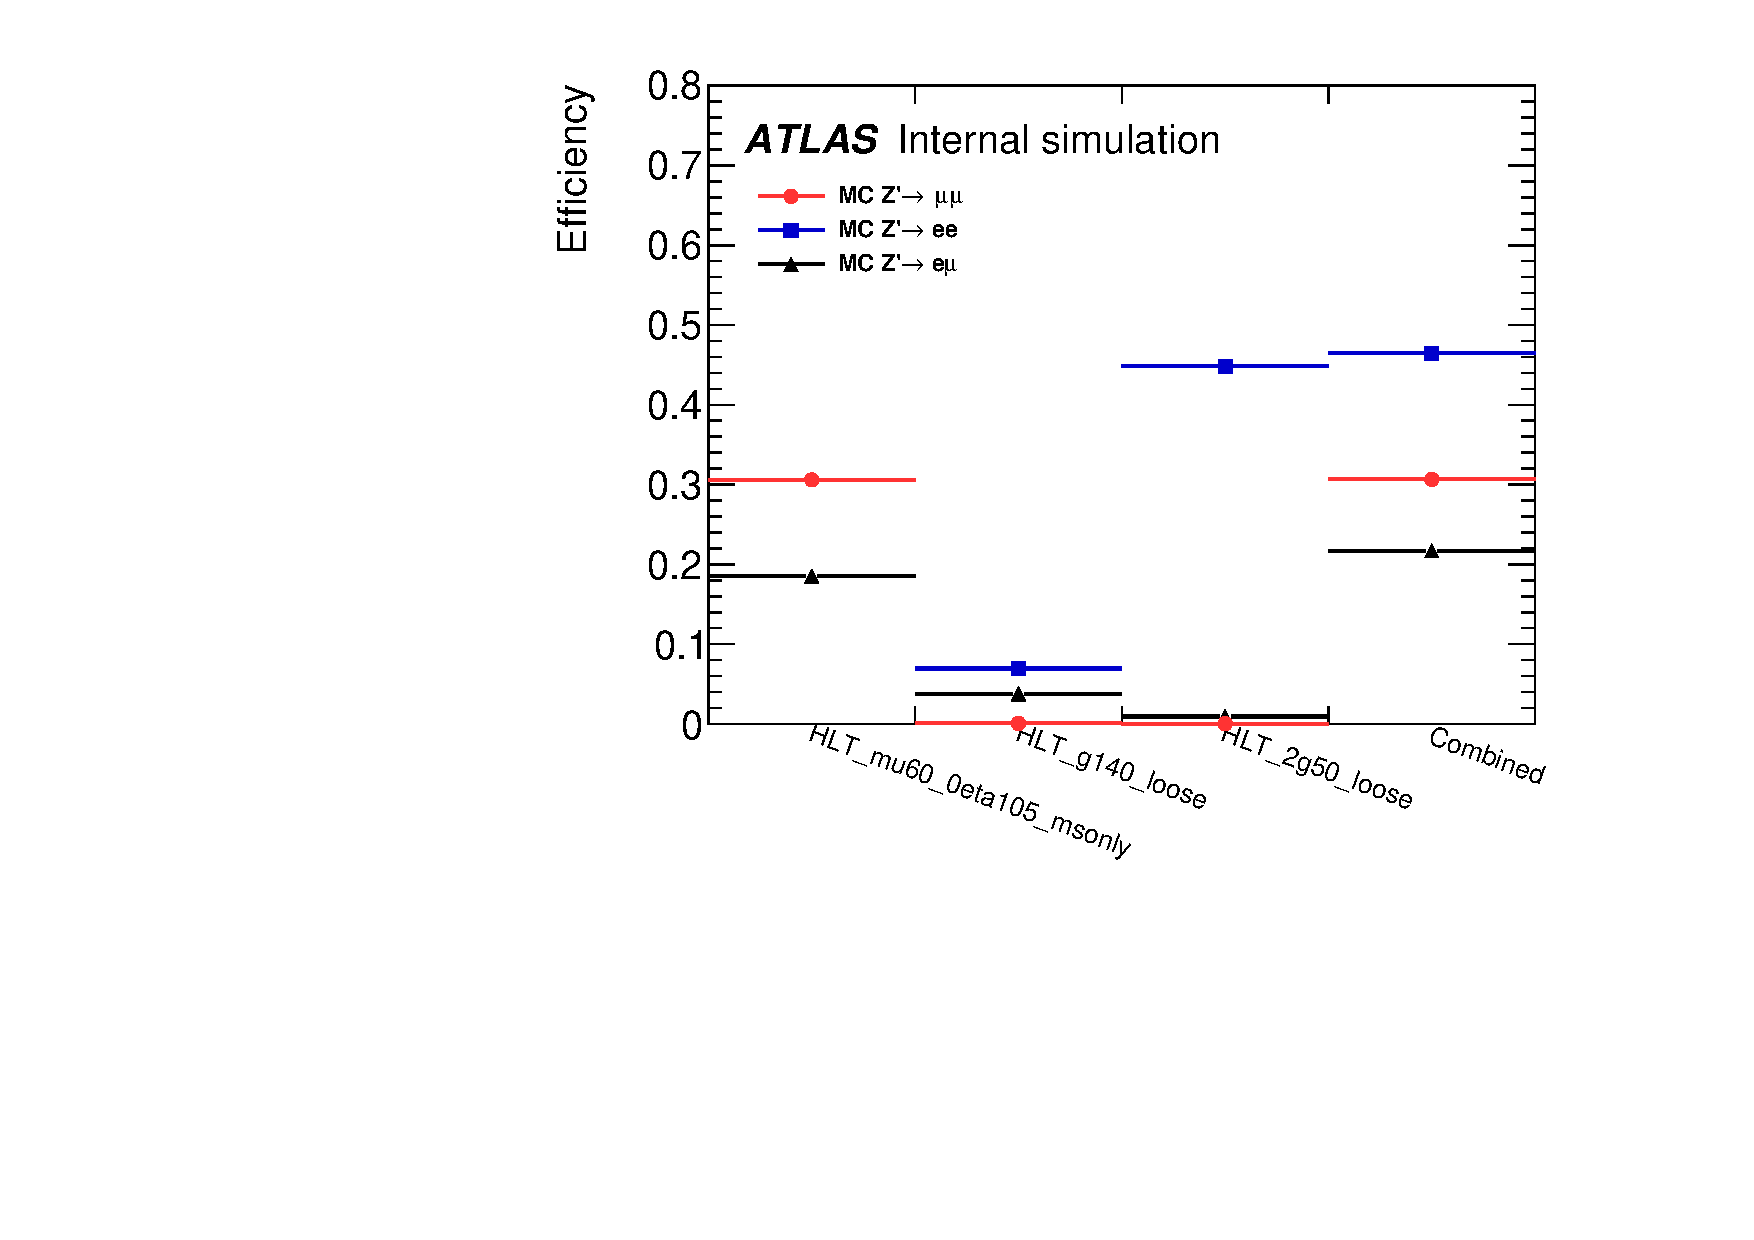
\includegraphics[width=0.50\textwidth]{figures/m_dv_eff_trig_allchannel.pdf}
	\centering
	\caption{Trigger efficiency of single muon, single photon, di-photon, and the combined triggers of the signal MC samples of $Z'\rightarrow\mumu, \ee$, and \emu generated with $m=$ 250 GeV and $c\tau=$ 250 mm.}
	\label{fig:m_trig_eff_allchannel}
\end{figure}

The trigger efficiency on all \mumu signal MC samples is shown in Table~\ref{table:m_trig_eff_mumu}. It is evident that at low $Z'$ mass ($\sim$100 GeV), the combined trigger efficiency on the signal MC sample is significantly reduced because the typical $p_{T}$ of the signal muons is lower than the $p_{T}$ threshold of the single muon trigger.

The trigger study indicates that there is a substantial loss in the signal efficiency at trigger level before reconstruction, and developing dedicated, more efficient triggers for long-lived particles will provide potential improvement in sensitivity to long-lived particles. The systematic uncertainties in trigger efficiency is estimated by tag-and-probe method in Section~\ref{sec:syst:trigger}.

\begin{table}[!htb]
  \centering
  \begin{tabular}{ c c | c c c c}
    \hline
    \hline
    %       &       & \multicolumn{4}{c}{$Z'\rightarrow\mumu$}                \\
    $m_{Z'}$ (GeV) & $c\tau$ (mm) & Single muon & Single photon & Di-photon & Combined \\
    \hline
    100			&	100	& 0.047 	& < 0.001   &0  	    &0.047  		\\
    100			&	250	& 0.043  	&0  	 	&0  	    &0.043  		\\
    100			&	500	& 0.039 	&0  	 	&0  	    &0.039  		\\
    250			&	100	& 0.343  	&< 0.001 	&< 0.001    &0.344  		\\
    250			&	250	& 0.306  	&< 0.001 	&< 0.001    &0.307  		\\
    250			&	500	& 0.230 	&< 0.001 	&< 0.001    &0.230  		\\
    500			&	100	& 0.454 	&0.010   	&< 0.001    &0.459  		\\
    500			&	250	& 0.410 	&0.009   	&< 0.001    &0.415  		\\
    500			&	500	& 0.331  	&0.008   	&0.001      &0.336  		\\
    750			&	100	& 0.541 	&0.026   	&0.002      &0.553  		\\
    750			&	250	& 0.470 	&0.023   	&0.003      &0.481  		\\
    750			&	500	& 0.391 	&0.022 	    &0.001      &0.402  		\\
    1000	    &	100	& 0.570   	&0.039   	&0.004      &0.586  		\\
    1000	    &	250	& 0.512   	&0.036   	&0.003      &0.526  		\\
    1000	    &	500	& 0.430   	&0.034 	    &0.004      &0.444  		\\
    \hline
    \hline
  \end{tabular}
  \caption{Trigger efficiency of single muon, single photon, di-photon triggers, and the combined trigger efficiency on the signal MC samples of $Z'\rightarrow\mumu$.}
  \label{table:m_trig_eff_mumu}
\end{table}

\section{Lepton reconstruction efficiency}
\label{sec:tracking_efficiency}
The tracking efficiency, $\varepsilon_{\mathrm{track}}$, and the lepton identification efficiency, $\varepsilon_{\mathrm{lepton}}$, are studied together as a lepton reconstruction efficiency. The lepton reconstruction efficiency is defined and estimated as follows. From a signal MC sample, the leptons decaying from $Z'$ are collected at generator-level, referred as \textit{truth} signal leptons. For each truth signal lepton, if there is a reconstructed lepton with its ID track matched to the ID track of the truth signal lepton by a hit-based truth matching scheme, it is marked as reconstructed. The ratio of reconstructed signal leptons to the total number of signal leptons produced in the sample is taken as the lepton reconstruction efficiency. No \texttt{RPVLL} or trigger filter is applied in estimating the lepton reconstruction efficiency.

Figure~\ref{fig:lepton_eff} shows the representative plot of the lepton reconstruction efficiency as a function of track parameters using the combined signal MC samples of $Z'$ decaying to all three channels, generated with $m = $ 250 GeV and $c\tau=$ 250 mm.

\begin{figure}[!htb]
    \centering
    \subfloat[]{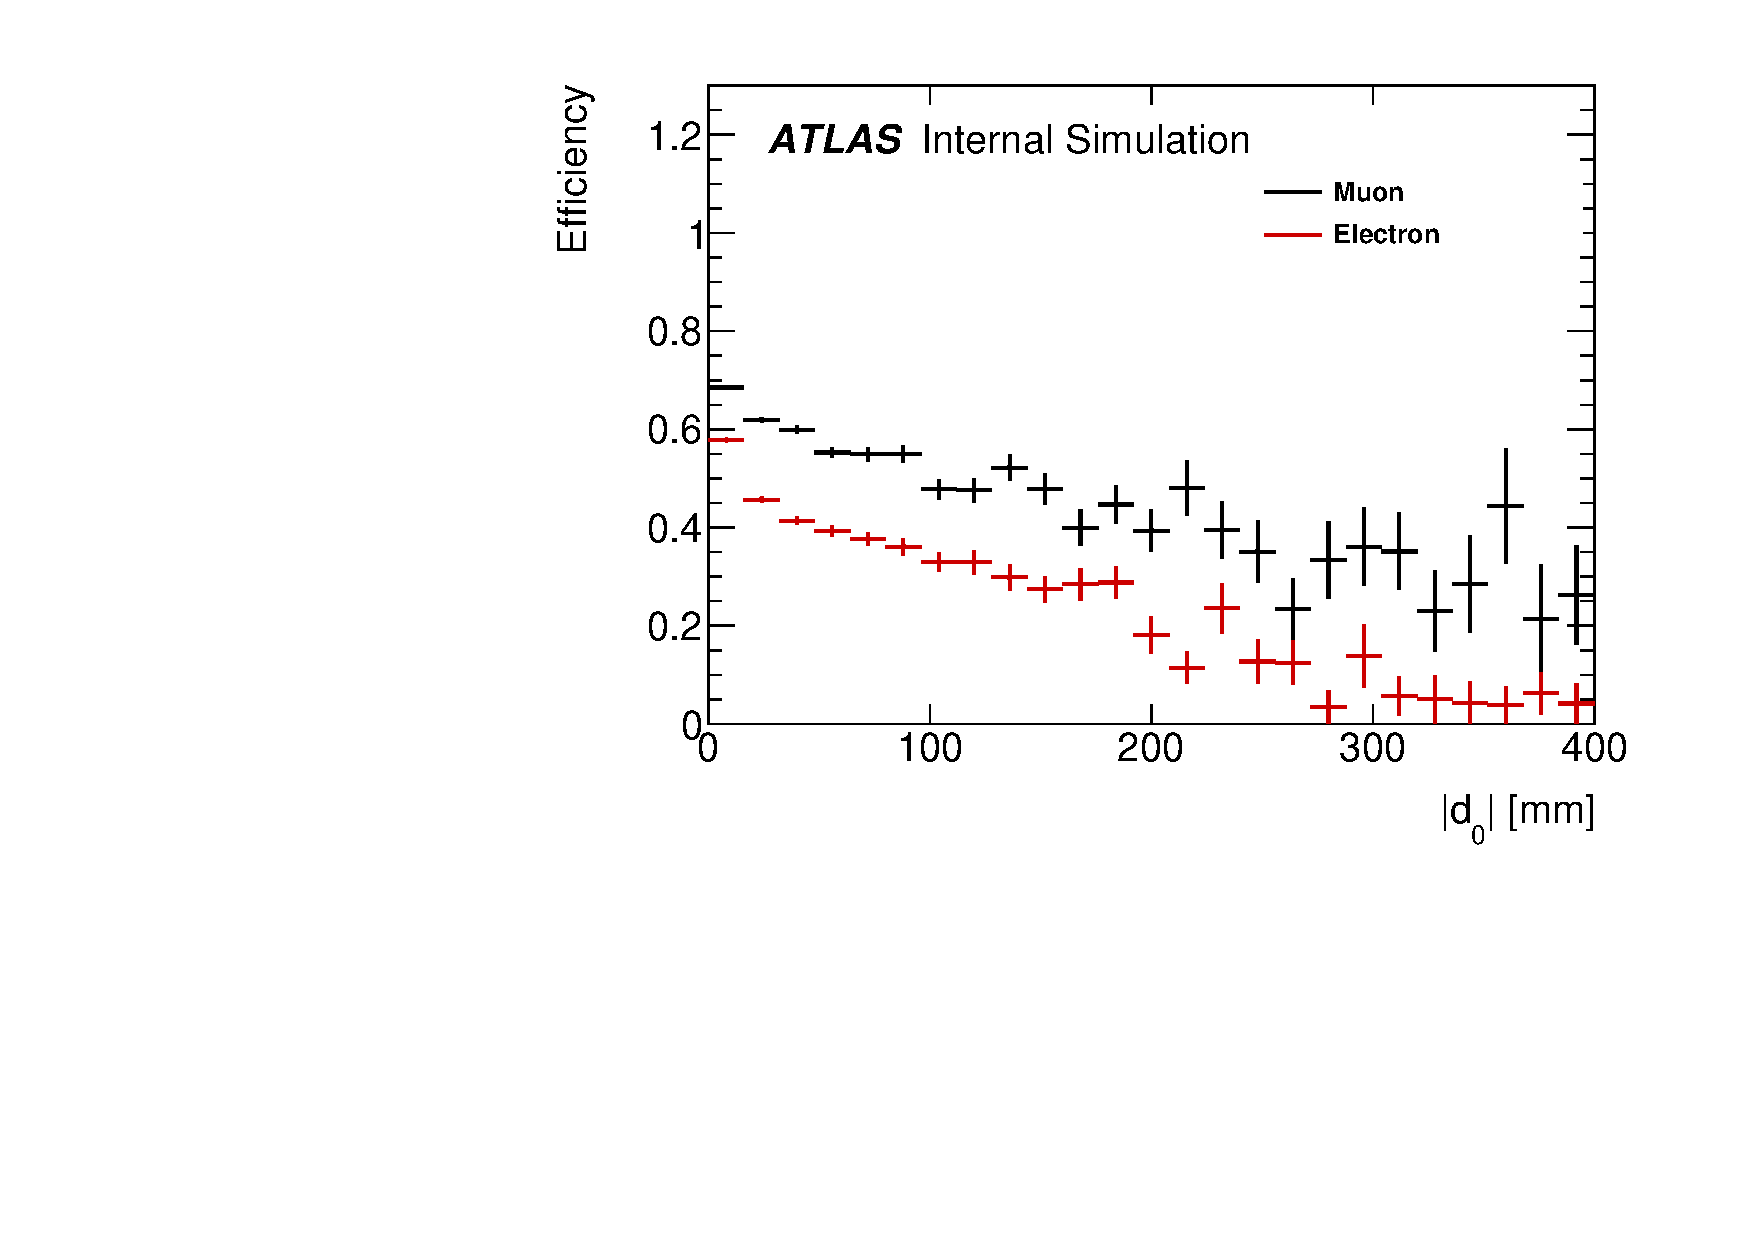
\includegraphics[width=0.50\textwidth]{figures/m_lepton_efficiency_d0.pdf}}
    \subfloat[]{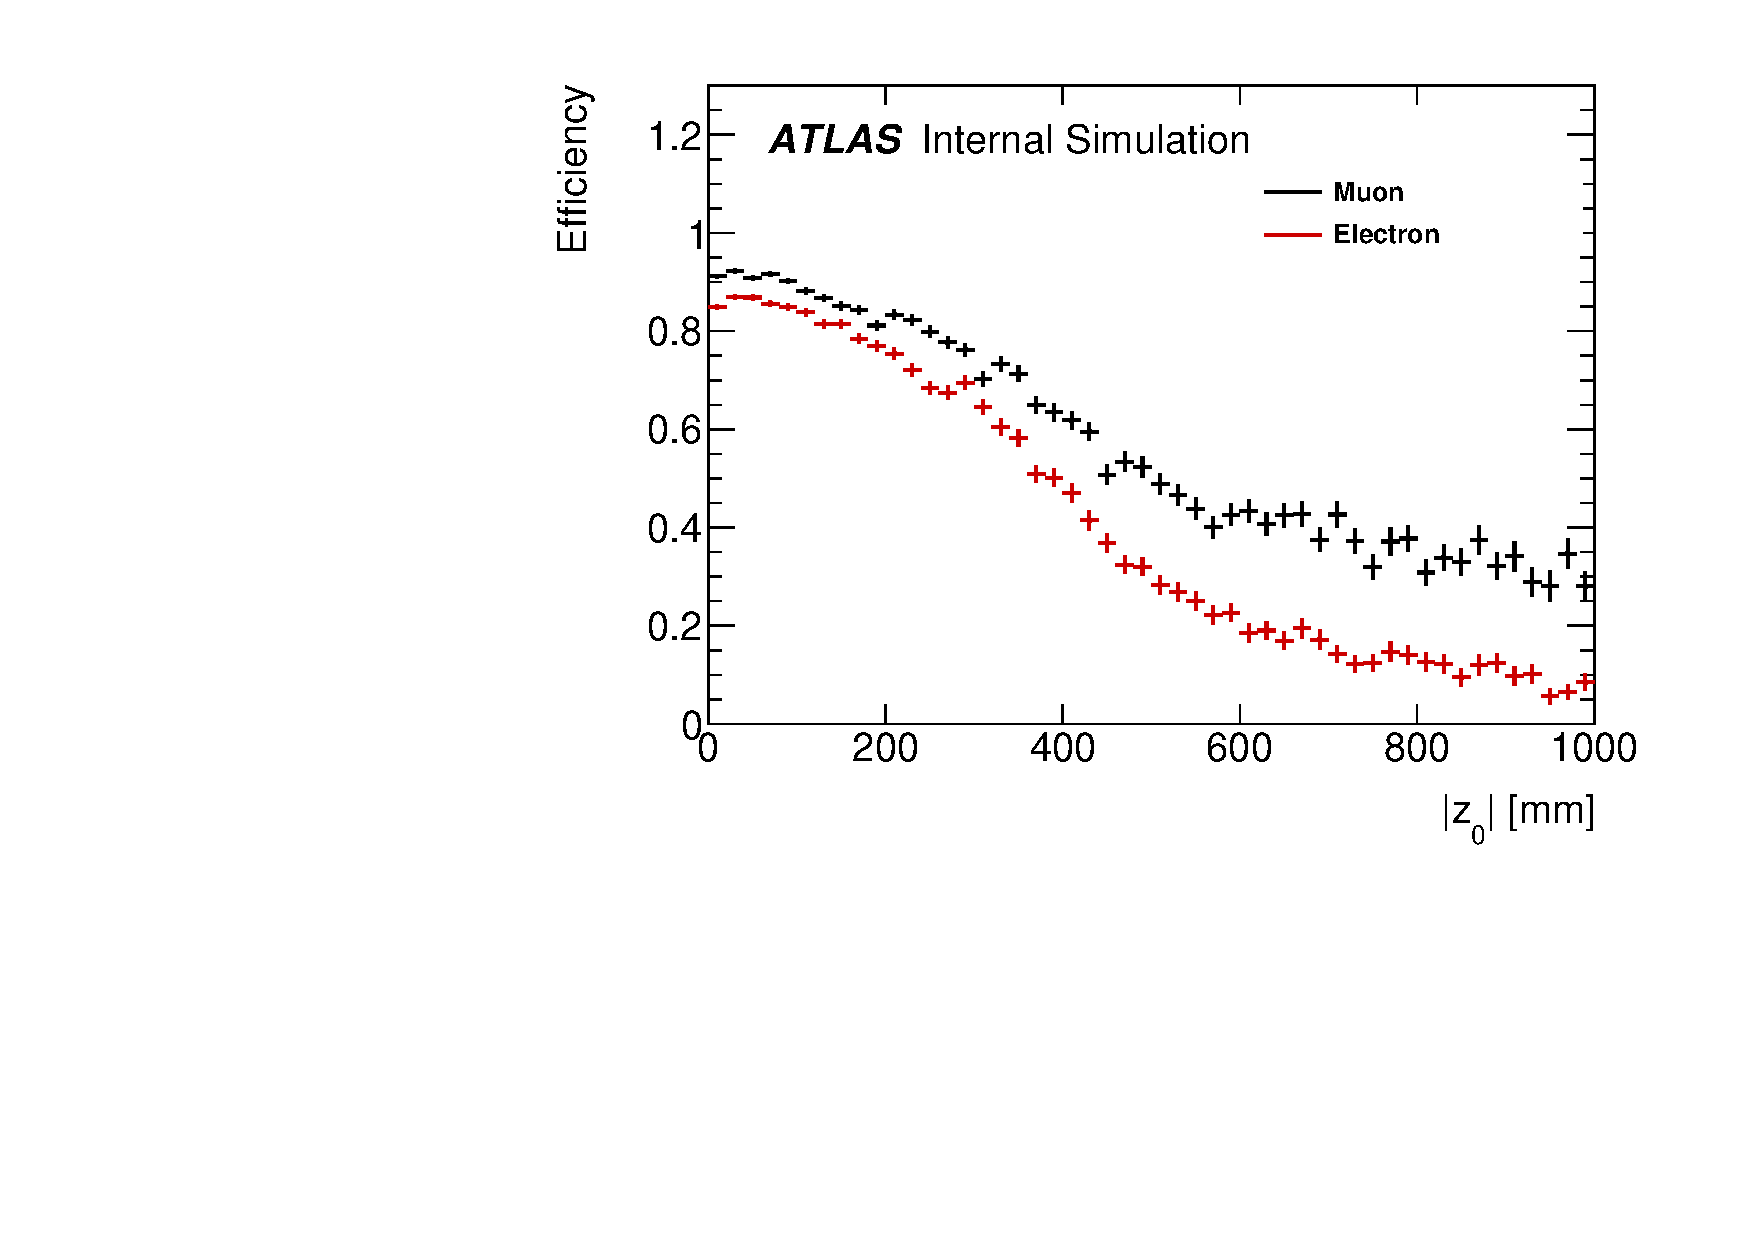
\includegraphics[width=0.50\textwidth]{figures/m_lepton_efficiency_z0.pdf}} \\
    \subfloat[]{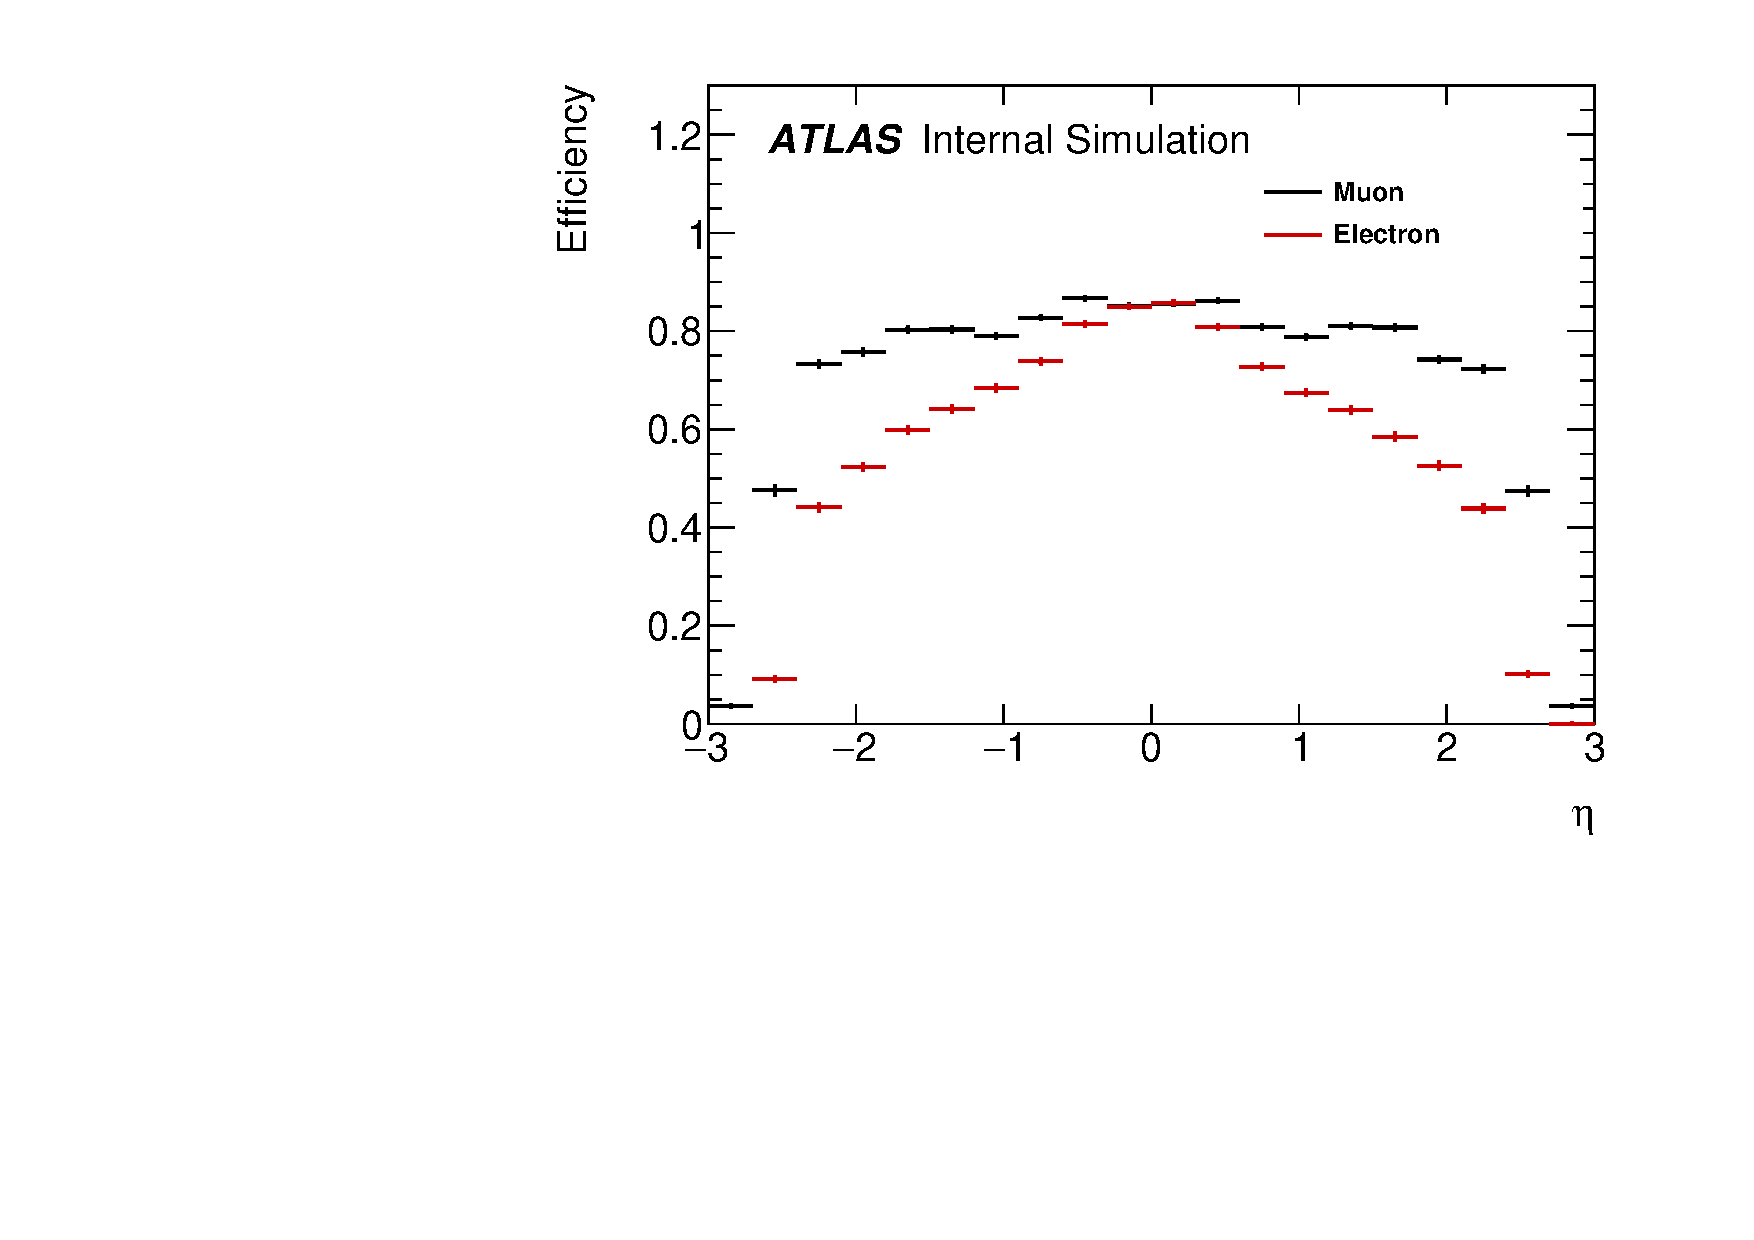
\includegraphics[width=0.50\textwidth]{figures/m_lepton_efficiency_eta.pdf}}
    \subfloat[]{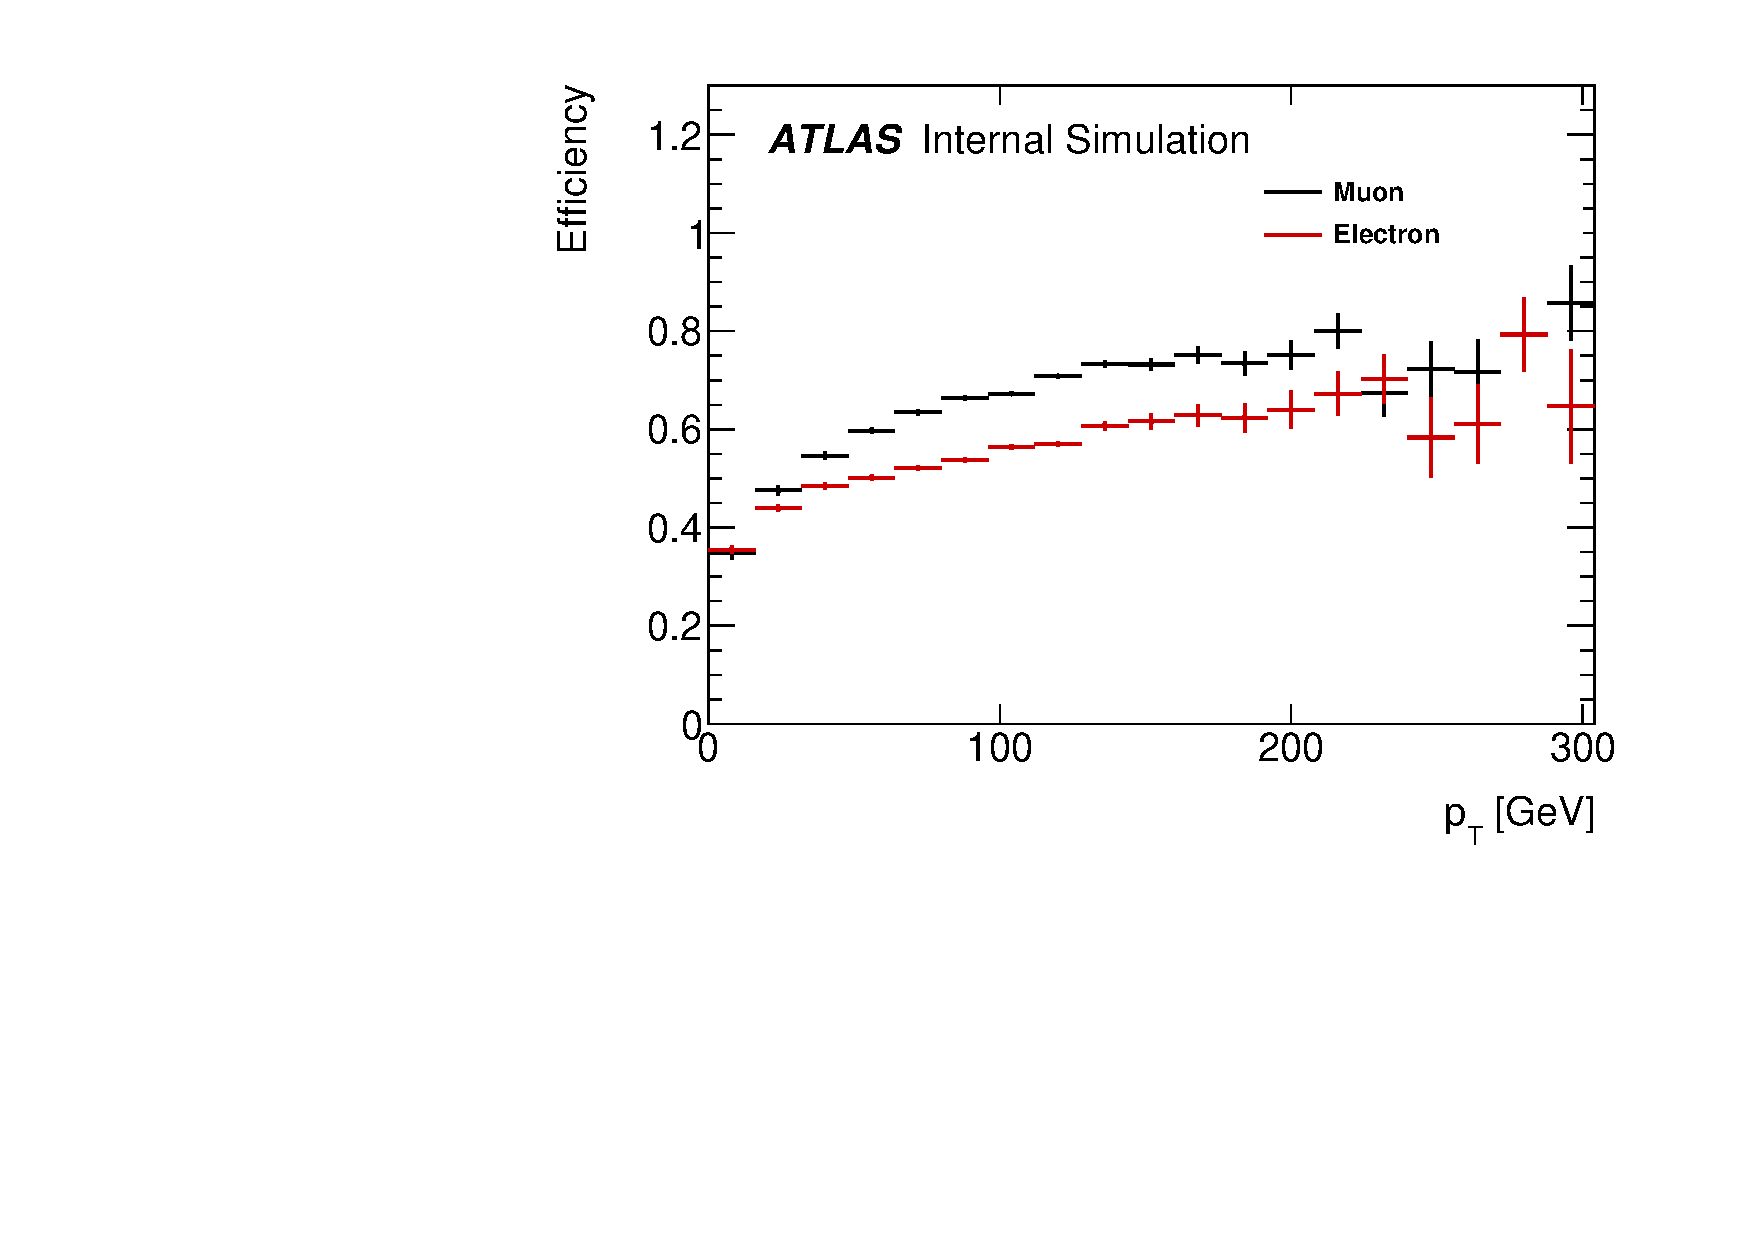
\includegraphics[width=0.50\textwidth]{figures/m_lepton_efficiency_pt.pdf}} 
    \caption{Lepton reconstruction efficiency as a function of (a) $d_{0}$, (b) $z_{0}$, (c) $\eta$, and (d) $p_{T}$ of signal leptons using the signal MC sample generated with $m=$ 250 GeV and $c\tau=$ 250 mm.}
    \label{fig:lepton_eff}
\end{figure}

It is evident that the efficiency drops drastically at $\eta > 2.0$ where the Pixel barrel region ends due to the minimum silicon hits requirement on tracks as shown in Table~\ref{table:tracking}. The efficiency is not very sensitive to $p_{T}$ except low $p_{T}$ region ($p_{T} < 20$).

The lepton reconstruction efficiency decreases for large $d_{0}$ and $z_{0}$. In the signal MC samples, most of $Z'$ decay within the Pixel barrel region, $r < $ 122.5 mm and $z < $ 400.5 mm, where the lepton reconstruction efficiency is high.

\section{Overall reconstruction efficiency}
\label{sec:combined_reco_efficiency}
The overall reconstruction efficiency represents the signal efficiency defined in Eq.~\ref{eq:OverallEff}, i.e. the ratio of $Z'$s reconstructed as displaced vertices in the signal region to the total $Z'$ produced in the sample. In this section, the signal selection cut flows (Section~\ref{sec:signal_cutflow}), the signal efficiency, and the efficiency distributions (Section~\ref{sec:efficiency}) are presented. In Section~\ref{sec:efficiency_map}, efficiency maps of the signal samples are presented as a function of $p_{T}$, $\eta$ of $Z'$.

\subsection{Event and vertex cut flow}
\label{sec:signal_cutflow}
The signal MC samples are processed as described in Section~\ref{sec:selection:pre}, in which long-lived $Z'$s are reconstructed as secondary vertices. The event and the vertex selections (Table~\ref{table:signal_selection}) are applied to the processed samples, and representative plots of these event vertex cut flow are shown in Figure~\ref{fig:signal_cutflow_MC_mumu} using the signal MC samples of $Z'$ decaying to \mumu generated with $m=$ 250, 1000 GeV for $c\tau=$ 100 mm.

\begin{figure}[!htb]
    \centering
    \subfloat[]{\label{subfig:event_cutflow_MC}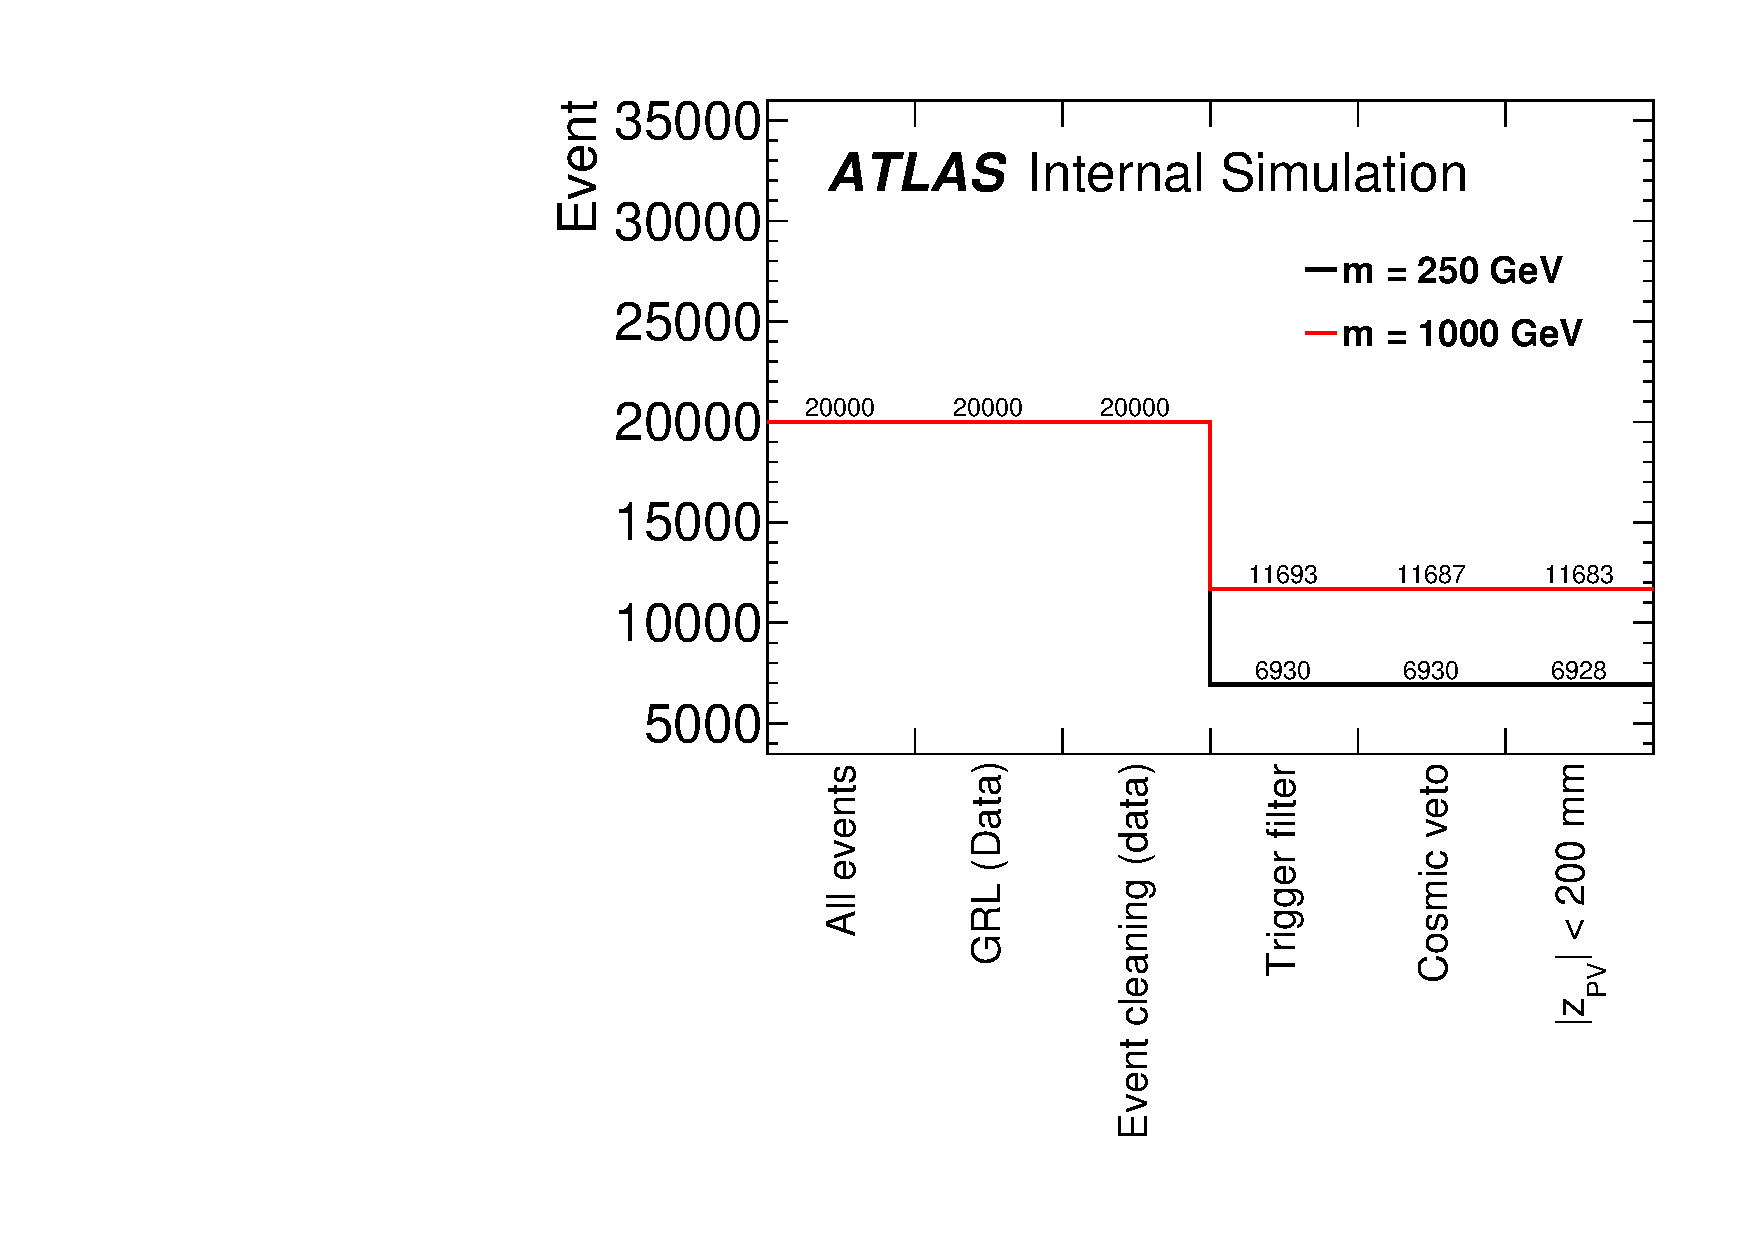
\includegraphics[width=0.50\textwidth]{figures/m_event_cutflow_MC_mumu.pdf}}
    \subfloat[] {\label{subfig:vertex_cutflow_MC}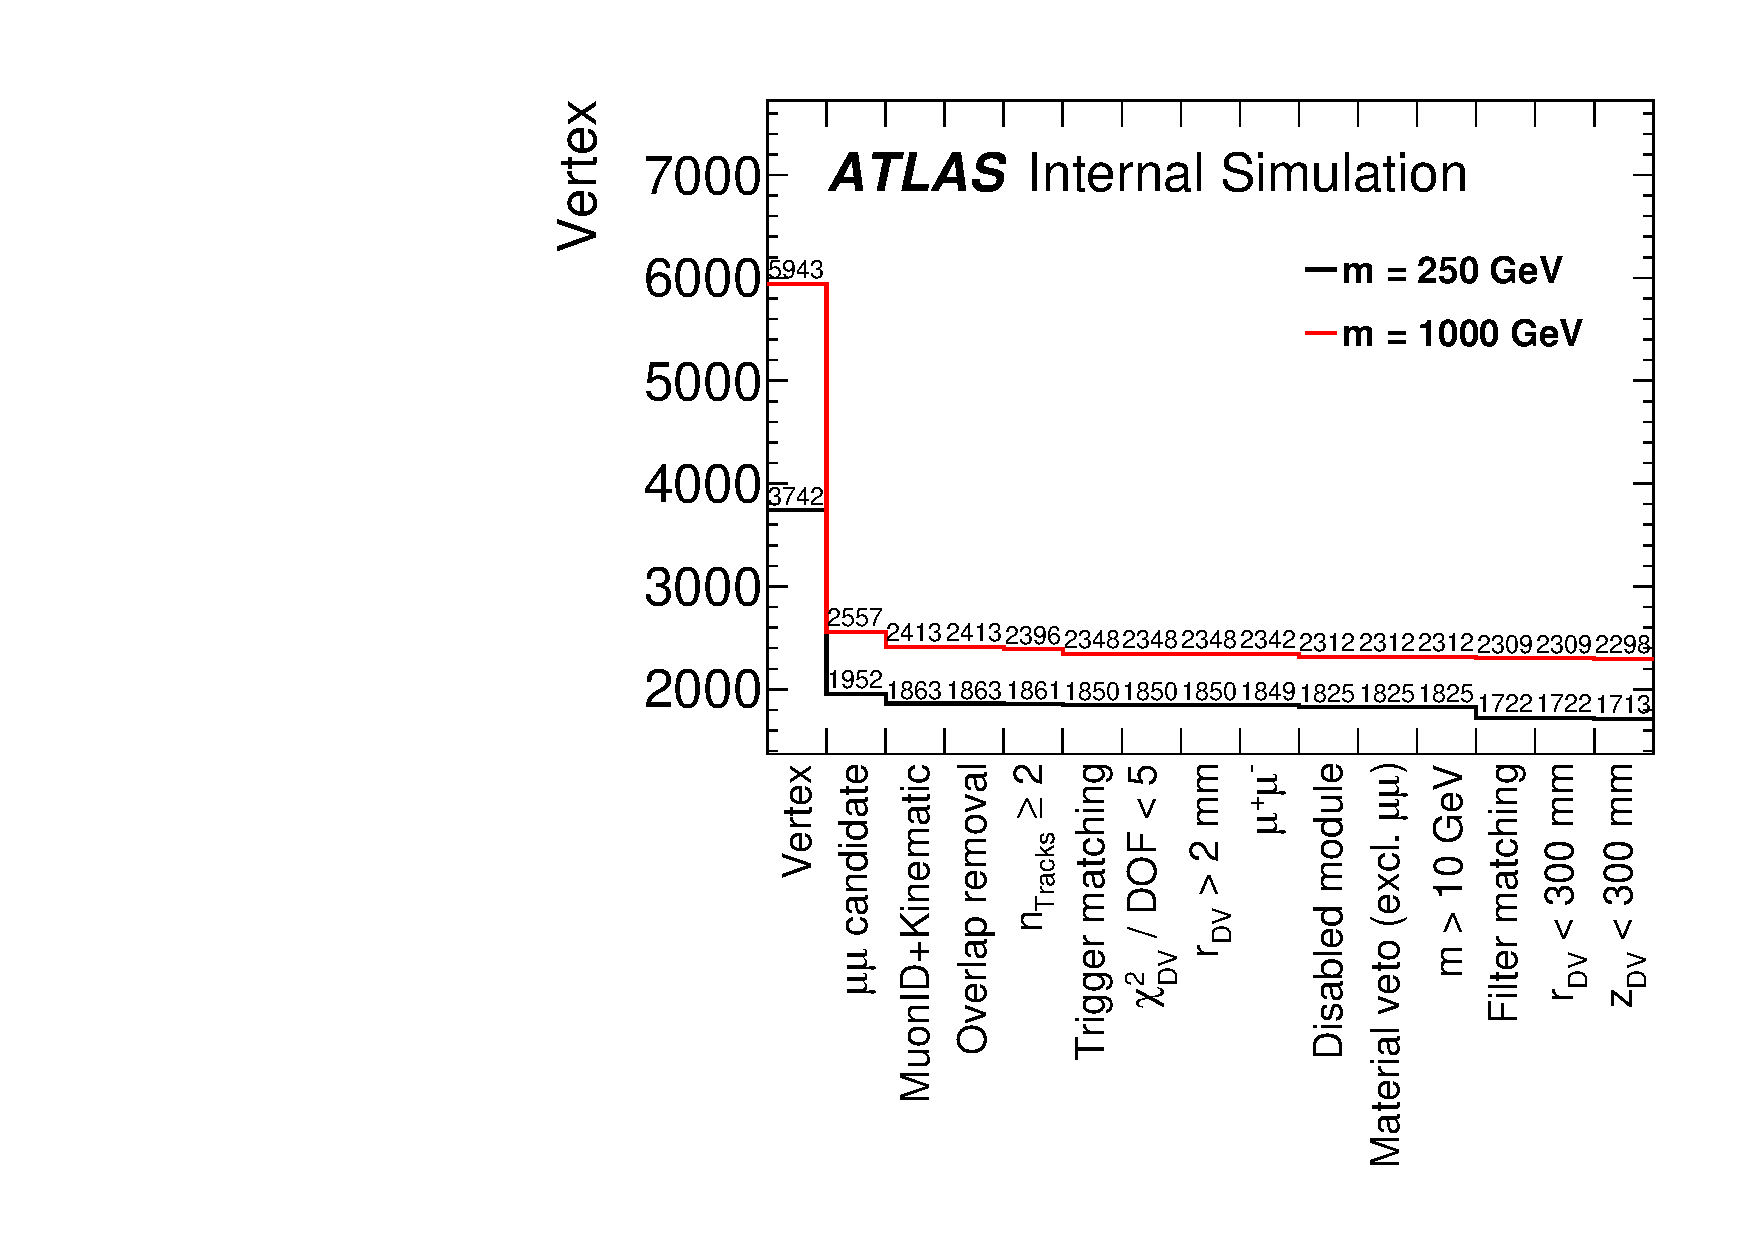
\includegraphics[width=0.50\textwidth]{figures/m_dv_cutflow_MC_mumu.pdf}} \\
    \caption{(a) Event cut flow, and (b) vertex cut flow using the signal MC samples of $Z'\rightarrow \mumu$ generated with $m =$ 500,1000 GeV for $c\tau= $ 100 mm.}
    \label{fig:signal_cutflow_MC_mumu}
\end{figure}

In the event cut flow, \texttt{GoodRunsList} filter and Event cleaning are shown as place holders as they are only applied to data sample. About 34-60$\%$ of signal events passed the event cut flow, but the vertex cut flow shows that only about 18-25$\%$ of signal events have a displaced vertex candidate, indicating that there is a significant loss of signal efficiency in the vertex reconstruction process. The following selection criteria, $\chi^{2} /$ DOF $<$ 5 and the minimum displacement cut ($r > $ 2 mm), are applied, but the effect is very small as expected because the same requirements are applied in the secondary vertex reconstruction algorithm. Material veto is applied to all vertex types except \mumu vertex. The minimum dilepton mass requirement has minimum impact on the signal efficiency.

Events and vertex cut flow of other signal samples are available in Table~\ref{table:cutflow_all}.


\begin{sidewaystable}[!htb]
  \centering
  \resizebox{\textwidth}{!}{
  \subfloat[$Z'\rightarrow \mumu$][]{
  \begin{tabular}{ c c c c c c c c c c c c c c c c c c c c c}
    \hline
    \hline
    $m_{Z'}$ (GeV) & $c\tau$ (mm)   & \rot{All events} 
                                    & \rot{Trigger Filter} 
                                    & \rot{Cosmic veto} 
                                    & \rot{$Z_{PV}<200$ mm} 
                                    & \rot{Vertex} 
                                    & \rot{$N_{\mu} > 2$ }
                                    & \rot{Muon Selection} 
                                    & \rot{Overlap Removal}
                                    & \rot{$N_{\mu}=2$}
                                    & \rot{Trigger Matching}
                                    & \rot{$\chi^{2} /$ DOF $< 5$}
                                    & \rot{Disp. > 2 mm}
                                    & \rot{\mumu}
                                    & \rot{Disabled Module}
                                    & \rot{$m > 10$ GeV}
                                    & \rot{Filter Matching}
                                    & \rot{$R_{DV} < 300$ mm}
                                    & \rot{$z_{DV} < 300$ mm} \\
    \hline
    100&	250&	20000&	818&	818&	818&	533&	269&	260&	260&	260&	259&	259&	259&	259&	252&	252&	82&	82&	81 \\
    100&	500&	20000&	761&	761&	761&	416&	165&	154&	154&	154&	154&	154&	154&	154&	148&	148&	50&	50&	49 \\
    100&	100&	20000&	940&	940&	940&	644&	366&	342&	342&	339&	339&	339&	339&	339&	330&	330&	108&	108&	106 \\
    250&	250&	20000&	6180&	6179&	6176&	3467&	1809&	1708&	1708&	1703&	1700&	1700&	1700&	1699&	1677&	1677&	1605&	1605&	1582 \\
    250&	500&	20000&	4922&	4921&	4921&	2680&	1354&	1284&	1284&	1278&	1276&	1276&	1276&	1276&	1261&	1261&	1205&	1205&	1176 \\
    250&	100&	20000&	6930&	6930&	6928&	3742&	1952&	1863&	1863&	1861&	1850&	1850&	1850&	1849&	1825&	1825&	1722&	1722&	1713 \\
    500&	500&	20000&	6724&	6720&	6717&	3605&	1777&	1666&	1666&	1658&	1646&	1646&	1646&	1646&	1617&	1617&	1611&	1611&	1572 \\
    500&	250&	20000&	8273&	8272&	8269&	4481&	2191&	2080&	2080&	2068&	2056&	2056&	2056&	2054&	2024&	2024&	2023&	2023&	2007 \\
    500&	100&	19000&	9146&	9145&	9144&	4680&	2205&	2091&	2091&	2085&	2068&	2068&	2068&	2068&	2047&	2047&	2042&	2042&	2034 \\
    750&	100&	20000&	11032&	11028&	11027&	5605&	2473&	2330&	2330&	2313&	2282&	2282&	2282&	2281&	2267&	2267&	2254&	2254&	2250 \\
    750&	500&	20000&	8059&	8055&	8054&	4262&	2017&	1878&	1878&	1868&	1851&	1851&	1851&	1849&	1824&	1824&	1820&	1819&	1784 \\
    750&	250&	20000&	9622&	9616&	9613&	5301&	2626&	2457&	2457&	2441&	2421&	2421&	2421&	2419&	2391&	2391&	2386&	2385&	2364 \\
    1000&	250&	20000&	10517&	10515&	10514&	5804&	2725&	2578&	2578&	2564&	2518&	2518&	2517&	2512&	2479&	2479&	2476&	2476&	2457 \\
    1000&	100&	20000&	11693&	11687&	11683&	5943&	2557&	2413&	2413&	2396&	2348&	2348&	2348&	2342&	2312&	2312&	2309&	2309&	2298 \\
    1000&	500&	20000&	8905&	8902&	8901&	4878&	2295&	2170&	2170&	2155&	2129&	2129&	2129&	2117&	2092&	2092&	2089&	2089&	2058 \\
    \hline
    \hline
  \end{tabular}
  }}

  \caption{Event and vertex cut flow of signal samples}
  \label{table:cutflow_all}
\end{sidewaystable}

\begin{sidewaystable}[!htb]\ContinuedFloat
  \centering
  \resizebox{\textwidth}{!}{
  \subfloat[$Z'\rightarrow \mumu$][]{
  \begin{tabular}{ c c c c c c c c c c c c c c c c c c c c c c}
    \hline
    \hline
    $m_{Z'}$ (GeV) & $c\tau$ (mm)   & \rot{All events} 
                                    & \rot{Trigger Filter} 
                                    & \rot{Cosmic veto} 
                                    & \rot{$Z_{PV}<200$ mm} 
                                    & \rot{Vertex} 
                                    & \rot{$N_{e} > 2$ }
                                    & \rot{Electron Selection} 
                                    & \rot{Bad Cluster} 
                                    & \rot{Overlap Removal}
                                    & \rot{$N_{e}=2$}
                                    & \rot{Trigger Matching}
                                    & \rot{$\chi^{2} /$ DOF $< 5$}
                                    & \rot{Disp. > 2 mm}
                                    & \rot{\ee}
                                    & \rot{Disabled Module}
                                    & \rot{Material Veto}
                                    & \rot{$m > 10$ GeV}
                                    & \rot{Filter Matching}
                                    & \rot{$R_{DV} < 300$ mm}
                                    & \rot{$z_{DV} < 300$ mm} \\
    \hline
    100&	250&	20000&	323&	323&	323&	145&	61&	59&	58&	56&	56&	56&	56&	56&	56&	55&	36&	36&	15&	15&	15 \\
    100&	500&	20000&	241&	241&	241&	111&	31&	30&	29&	29&	29&	27&	27&	27&	27&	26&	19&	19&	10&	10&	9 \\
    100&	100&	20000&	315&	315&	315&	166&	71&	69&	69&	67&	67&	66&	66&	66&	66&	65&	52&	52&	16&	16&	15 \\
    250&	250&	20000&	9276&	9274&	9272&	4083&	1576&	1519&	1501&	1477&	1458&	1453&	1453&	1453&	1448&	1417&	1206&	1206&	1174&	1174&	1163 \\
    250&	500&	20000&	7755&	7750&	7749&	3203&	1105&	1063&	1057&	1038&	1017&	1011&	1011&	1011&	1007&	987&	803&	803&	769&	769&	758 \\
    250&	100&	20000&	10147&	10145&	10144&	4472&	1696&	1658&	1639&	1618&	1601&	1585&	1585&	1585&	1577&	1563&	1378&	1378&	1345&	1345&	1339 \\
    500&	500&	19000&	12279&	12278&	12276&	5029&	1566&	1505&	1502&	1493&	1471&	1466&	1466&	1466&	1455&	1432&	1194&	1194&	1185&	1185&	1162 \\
    500&	250&	20000&	14855&	14853&	14849&	6245&	1986&	1907&	1892&	1880&	1858&	1858&	1858&	1857&	1844&	1824&	1580&	1580&	1569&	1569&	1559 \\
    500&	100&	20000&	16012&	16008&	16006&	6621&	2017&	1940&	1925&	1900&	1878&	1877&	1877&	1877&	1857&	1843&	1668&	1668&	1656&	1656&	1652 \\
    750&	100&	20000&	18014&	18011&	18006&	7422&	2266&	2196&	2182&	2173&	2138&	2138&	2138&	2138&	2092&	2085&	1919&	1919&	1914&	1914&	1913 \\
    750&	500&	20000&	15290&	15286&	15283&	6206&	1853&	1791&	1778&	1768&	1731&	1731&	1731&	1731&	1711&	1690&	1423&	1423&	1419&	1419&	1399 \\
    750&	250&	20000&	16920&	16914&	16912&	7165&	2260&	2186&	2177&	2168&	2129&	2129&	2129&	2129&	2099&	2081&	1832&	1832&	1824&	1824&	1808 \\
    1000&	250&	20000&	17890&	17883&	17877&	7674&	2487&	2412&	2401&	2395&	2349&	2349&	2349&	2349&	2320&	2298&	2070&	2070&	2067&	2067&	2050 \\
    1000&	100&	20000&	18723&	18719&	18714&	7749&	2347&	2271&	2247&	2235&	2195&	2195&	2195&	2195&	2162&	2151&	2004&	2004&	1996&	1996&	1992 \\
    1000&	500&	19000&	15666&	15660&	15658&	6507&	1956&	1881&	1870&	1866&	1842&	1842&	1842&	1842&	1812&	1797&	1562&	1562&	1559&	1559&	1548 \\
    \hline
    \hline
  \end{tabular}
  }}
  \caption{Event and vertex cut flow of signal samples}
  \label{table:cutflow_all}
\end{sidewaystable}

\begin{sidewaystable}[!htb]\ContinuedFloat
  \centering
  \resizebox{\textwidth}{!}{
  \subfloat[$Z'\rightarrow \mumu$][]{
  \begin{tabular}{ c c c c c c c c c c c c c c c c c c c c c c}
    \hline
    \hline
    $m_{Z'}$ (GeV) & $c\tau$ (mm)   & \rot{All events} 
                                    & \rot{Trigger Filter} 
                                    & \rot{Cosmic veto} 
                                    & \rot{$Z_{PV}<200$ mm} 
                                    & \rot{Vertex} 
                                    & \rot{$N_{e} > 2$ }
                                    & \rot{Electron Selection} 
                                    & \rot{Bad Cluster} 
                                    & \rot{Overlap Removal}
                                    & \rot{$N_{e}=2$}
                                    & \rot{Trigger Matching}
                                    & \rot{$\chi^{2} /$ DOF $< 5$}
                                    & \rot{Disp. > 2 mm}
                                    & \rot{\ee}
                                    & \rot{Disabled Module}
                                    & \rot{Material Veto}
                                    & \rot{$m > 10$ GeV}
                                    & \rot{Filter Matching}
                                    & \rot{$R_{DV} < 300$ mm}
                                    & \rot{$z_{DV} < 300$ mm} \\
    \hline
    100&	250&	20000&	483&	483&	483&	255&	94&	91&	91&	89&	88&	88&	88&	88&	88&	87&	61&	61&	21&	21&	19 \\
    100&	500&	19000&	379&	379&	379&	178&	56&	53&	53&	53&	53&	53&	53&	53&	53&	50&	34&	34&	15&	15&	14 \\
    100&	100&	19000&	484&	484&	484&	295&	150&	145&	145&	137&	136&	134&	134&	134&	134&	127&	88&	88&	26&	26&	26 \\
    250&	250&	20000&	4273&	4272&	4265&	2251&	921&	901&	899&	874&	867&	848&	848&	848&	844&	829&	682&	682&	650&	650&	638 \\
    250&	500&	20000&	3486&	3484&	3481&	1667&	709&	695&	693&	678&	672&	663&	663&	663&	662&	653&	532&	532&	511&	511&	502 \\
    250&	100&	20000&	4771&	4769&	4768&	2326&	960&	938&	934&	899&	891&	868&	868&	868&	862&	851&	729&	729&	698&	698&	696 \\
    500&	500&	20000&	10885&	10883&	10883&	4797&	1732&	1697&	1689&	1623&	1604&	1595&	1594&	1594&	1581&	1552&	1327&	1327&	1264&	1264&	1239 \\
    500&	250&	20000&	12680&	12680&	12679&	5736&	2199&	2169&	2160&	2059&	2037&	2020&	2020&	2019&	2016&	1990&	1748&	1748&	1688&	1688&	1671 \\
    500&	100&	19000&	13351&	13349&	13346&	6049&	2168&	2135&	2131&	2040&	2019&	2005&	2005&	2005&	1999&	1981&	1793&	1793&	1736&	1736&	1728 \\
    750&	100&	19000&	16046&	16036&	16032&	7041&	2624&	2590&	2582&	2480&	2448&	2437&	2437&	2436&	2408&	2400&	2232&	2232&	2207&	2207&	2203 \\
    750&	500&	20000&	13598&	13590&	13585&	6033&	2170&	2132&	2125&	2025&	2003&	1995&	1995&	1995&	1983&	1965&	1686&	1686&	1644&	1644&	1604 \\
    750&	250&	20000&	15546&	15545&	15541&	7171&	2706&	2659&	2655&	2533&	2502&	2494&	2493&	2492&	2475&	2448&	2172&	2172&	2142&	2142&	2115 \\
    1000&	250&	20000&	16751&	16743&	16739&	7835&	3088&	3036&	3028&	2899&	2856&	2854&	2854&	2854&	2832&	2809&	2512&	2512&	2495&	2495&	2475 \\
    1000&	100&	18000&	15970&	15963&	15959&	7189&	2581&	2543&	2535&	2415&	2385&	2371&	2371&	2370&	2345&	2323&	2163&	2163&	2148&	2148&	2146 \\
    1000&	500&	19000&	14165&	14160&	14154&	6366&	2345&	2290&	2284&	2198&	2162&	2153&	2153&	2152&	2134&	2112&	1826&	1825&	1808&	1808&	1773 \\
    \hline
    \hline
  \end{tabular}
  }}
  \caption{Event and vertex cut flow of signal samples}
  \label{table:cutflow_all}
\end{sidewaystable}




\subsection{Signal efficiency and distribution}
\label{sec:efficiency}

The signal efficiency is studied by examining the efficiency distributions in the transverse ($r$), longitudinal ($z$) vertex position, and the angular distributions of the reconstructed vertices. The representative efficiency distributions are shown in Figure~\ref{fig:signal_vertex_dist} using the signal MC samples generated with $m =$500, 1000 GeV for $c\tau=$100 mm.

\begin{figure}[!htb]
    \centering
    \subfloat[]{\label{subfig:vertex_dist_r  }\includegraphics[width=0.49\textwidth]{figures/m_dv_efficiency_r.pdf}}
    \subfloat[]{\label{subfig:vertex_dist_z  }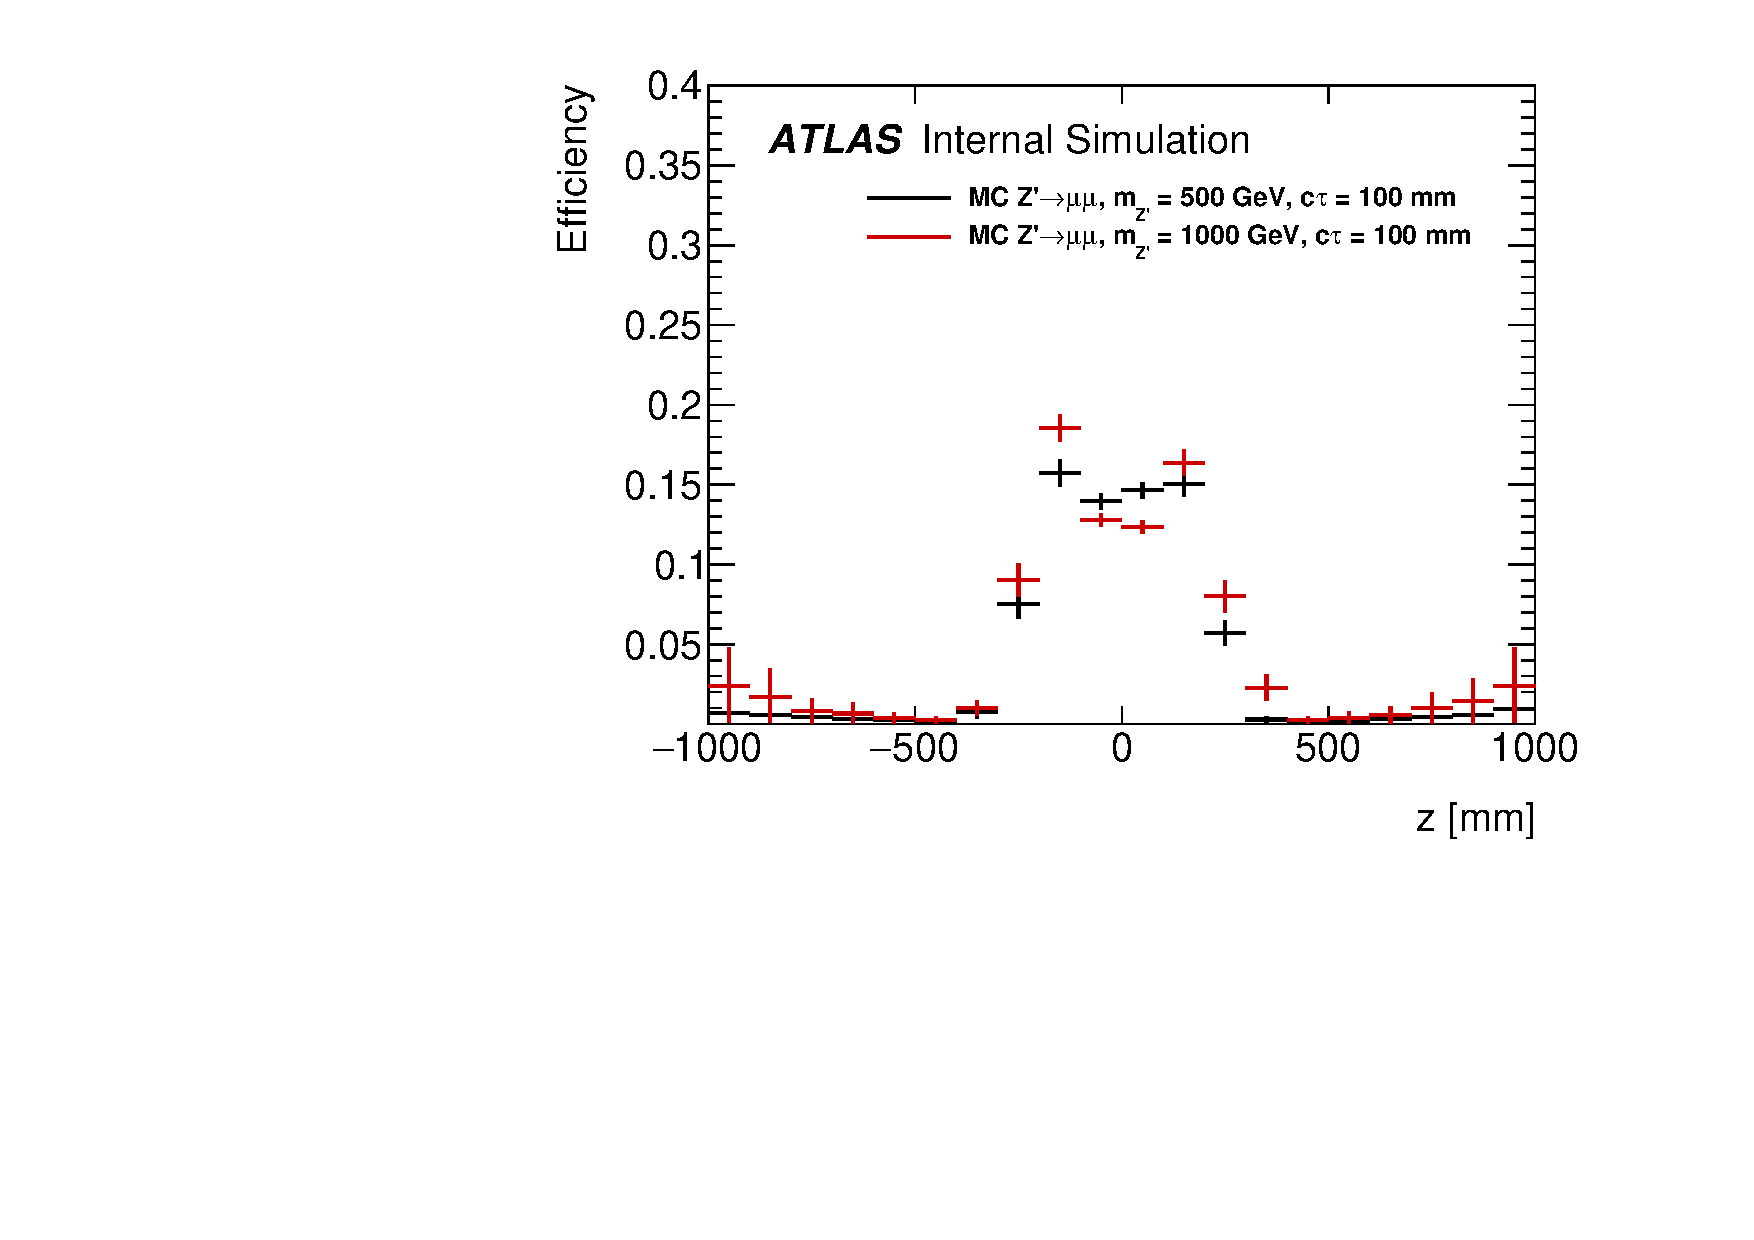
\includegraphics[width=0.49\textwidth]{figures/m_dv_efficiency_z.pdf}} \\
    \subfloat[]{\label{subfig:vertex_dist_eta}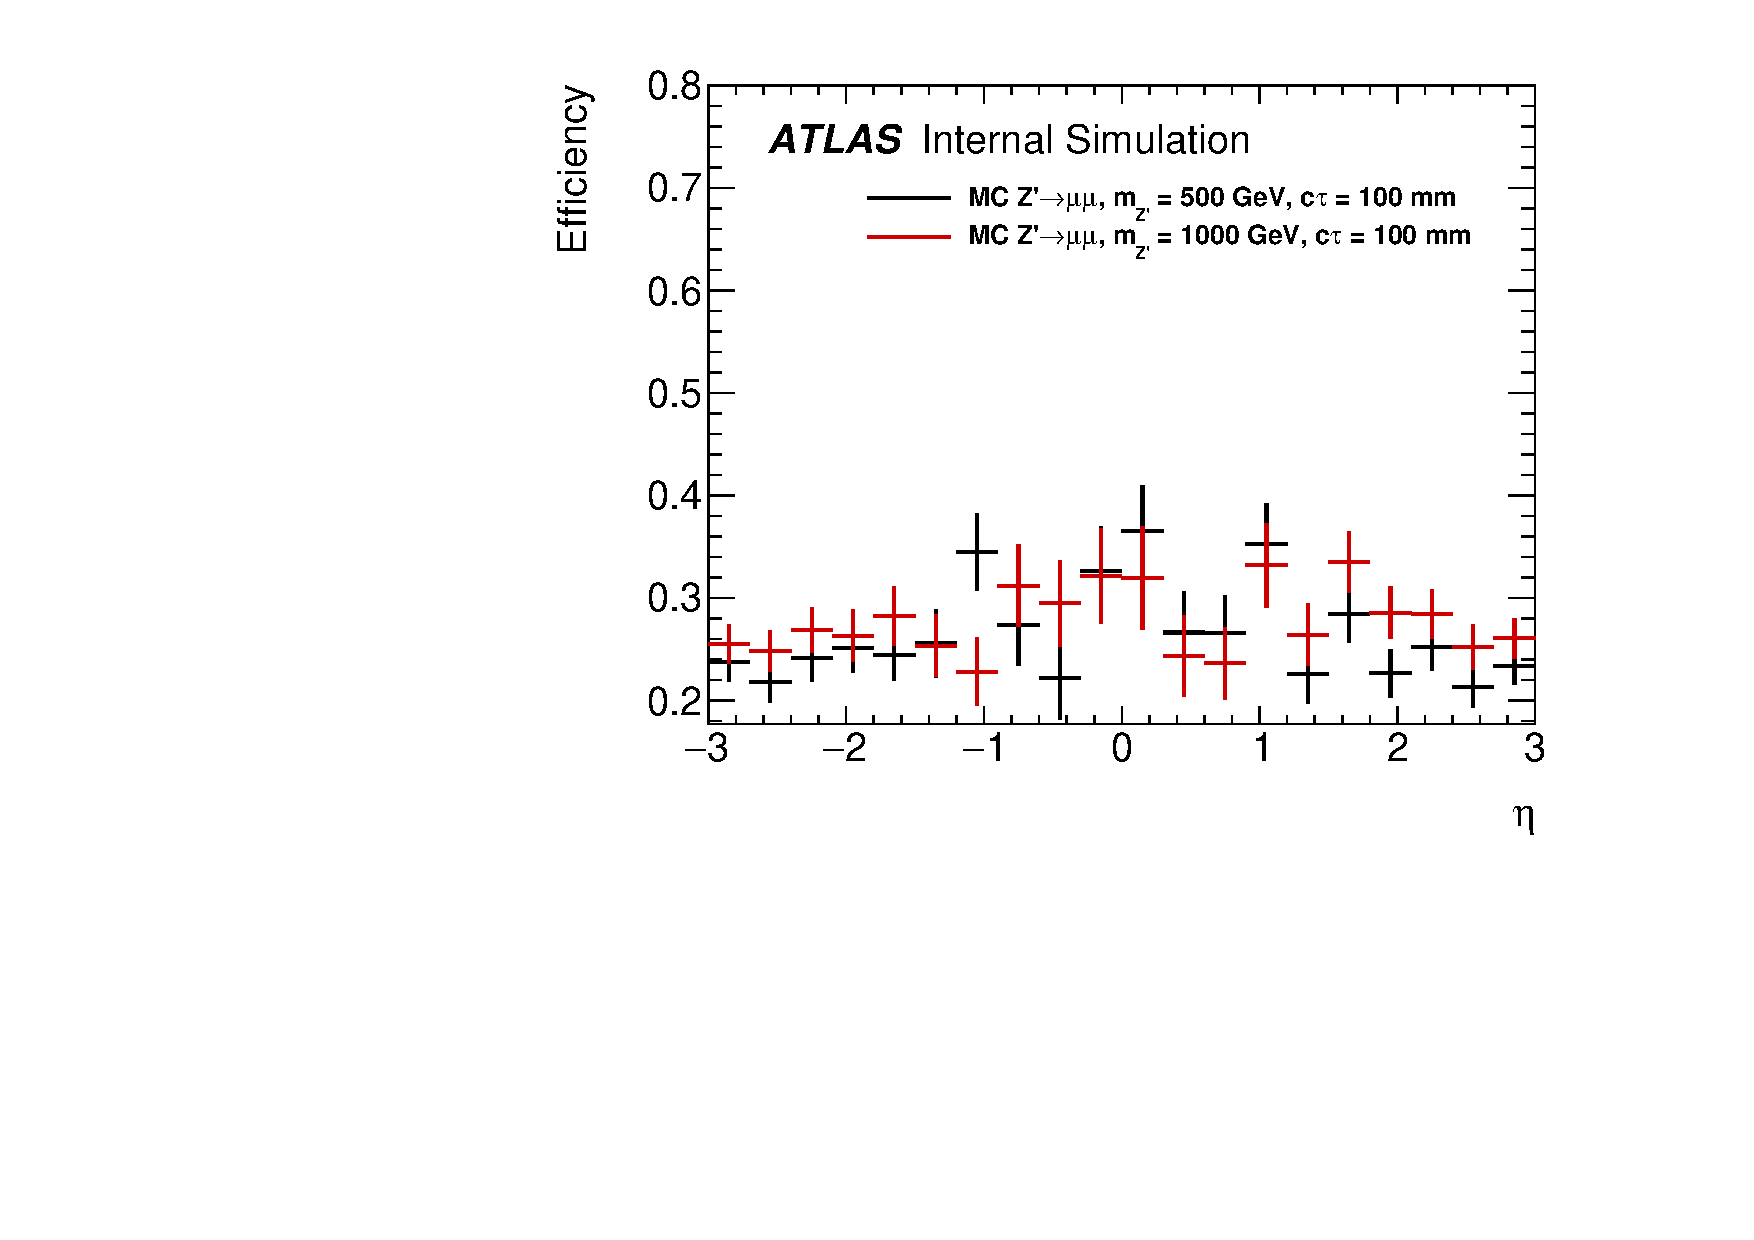
\includegraphics[width=0.49\textwidth]{figures/m_dv_efficiency_eta.pdf}}
    \subfloat[]{\label{subfig:vertex_dist_phi}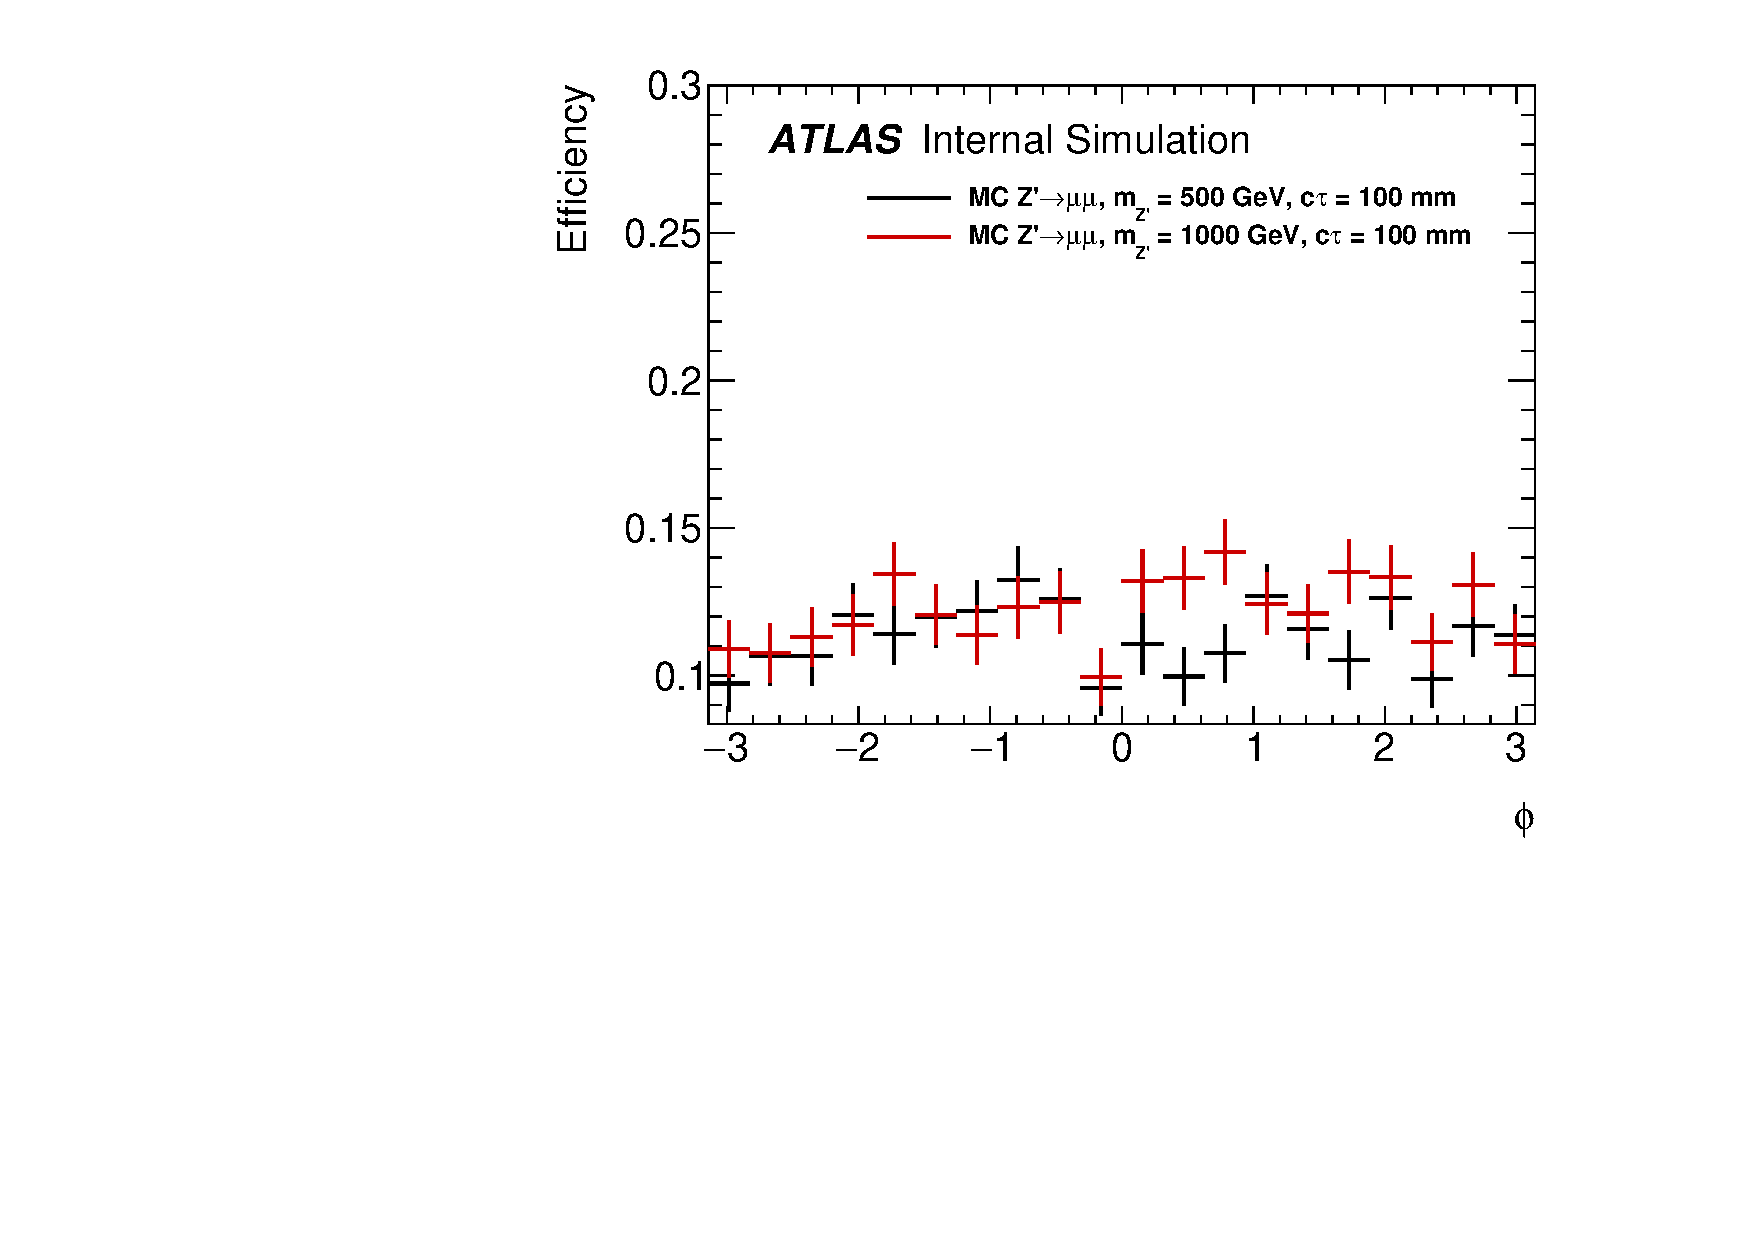
\includegraphics[width=0.49\textwidth]{figures/m_dv_efficiency_phi.pdf}} 
    \caption{Signal efficiency distributions in (a) $r$, (b) $z$, (c) $\eta$, and (d) $\phi$ of the signal MC samples of $Z'\rightarrow \mumu$ with $m=$ 500, 100 GeV for $c\tau=$ 100 mm.}
    \label{fig:signal_vertex_dist}
\end{figure}


The signal efficiency shows a significant dependence on vertex position which decreases at large $r$ and $z$ due to the minimum silicon hits requirement on tracks. The first bins in $r$ and $z$ distributions have lower efficiency due to the minimum displacement requirement ($r > $ 2 mm) on secondary vertices. The $r$ distribution shows features that reflects the physical structure of the ID. The $\eta$ distribution has higher efficiency in the central region, and the $\phi$ distribution is uniform as expected.

The overall signal efficiency for the signal samples are shown in Table~\ref{table:signal_eff}. The signal efficiency ranges from 14.9-33.3\% for mass above 500 GeV, but the efficiency is reduced for lower $Z'$ mass due to minimum $p_{T}$ thresholds on decaying leptons, especially for the samples with $m_{Z'}=100~\si{\GeV}$. The samples with shorter lifetime tend to have higher signal efficiency as expected. 

\begin{table}[!htb]
  \centering
  \begin{tabular}{ c c @{\hspace{1cm}} c @{\hspace{1cm}} c @{\hspace{1cm}} c }
    \hline
    \hline
    $m_{Z'}$ (GeV) & $c\tau$ (mm)   &$\mu\mu$  & $ee$  & $e\mu$ \\
    \hline
    100			   &  100	        &0.004	&0.001	&0.001   \\
    100			   &  250	        &0.002	&0.000	&0.001   \\
    100			   &  500	        &0.005	&0.001	&0.001   \\
    250			   &  100	        &0.079	&0.058	&0.032   \\
    250			   &  250	        &0.059	&0.038	&0.025   \\
    250			   &  500	        &0.086	&0.067	&0.035   \\
    500			   &  100	        &0.079	&0.061	&0.062   \\
    500			   &  250	        &0.100	&0.078	&0.084   \\
    500			   &  500	        &0.107	&0.083	&0.091   \\
    750			   &  100	        &0.113	&0.096	&0.116   \\
    750			   &  250	        &0.089	&0.070	&0.080   \\
    750			   &  500	        &0.118	&0.090	&0.106   \\
    1000	       &  100	        &0.123	&0.103	&0.124   \\
    1000	       &  250	        &0.115	&0.100	&0.119   \\
    1000	       &  500	        &0.103	&0.081	&0.093   \\
    \hline
    \hline
  \end{tabular}
  \caption{Overall signal efficiency of the signal samples.}
  \label{table:signal_eff}
\end{table}




\subsection{Efficiency map}
\label{sec:efficiency_map}
Signal efficiency for each mass and lifetime of long-lived $Z'$ sample is presented as a function of $p_{T}$ and $\eta$ of $Z'$. Because any neutral, LLP decaying to a dilepton pair can be mostly described by mass, lifetime, $p_{T}$, and $\eta$ of the LLP, these efficiency maps can be used for other BSM searches such as searching for long-lived neutralino in the context of SUSY R-parity violating theory.

Representative efficiency maps are shown in Figure~\ref{fig:signal_eff_map} using the signal MC samples of $Z' \rightarrow \mumu$ with $m=$ 500, 1000 GeV and $c\tau=$ 100, 500 mm. Although the overall signal efficiency is $\sim$10\% for these samples, the efficiencies in the central region of the efficiency maps are much higher because a large fraction of $Z'$ is produced in the forward region ($\eta > 2.5$) where no detector sensor is available for tracking, hence reducing the overall efficiency. Efficiency maps of other signal samples are available in Appendix~\ref{app:signal_efficiency_map}.

\begin{figure}[!htb]
    \centering
    \subfloat[]{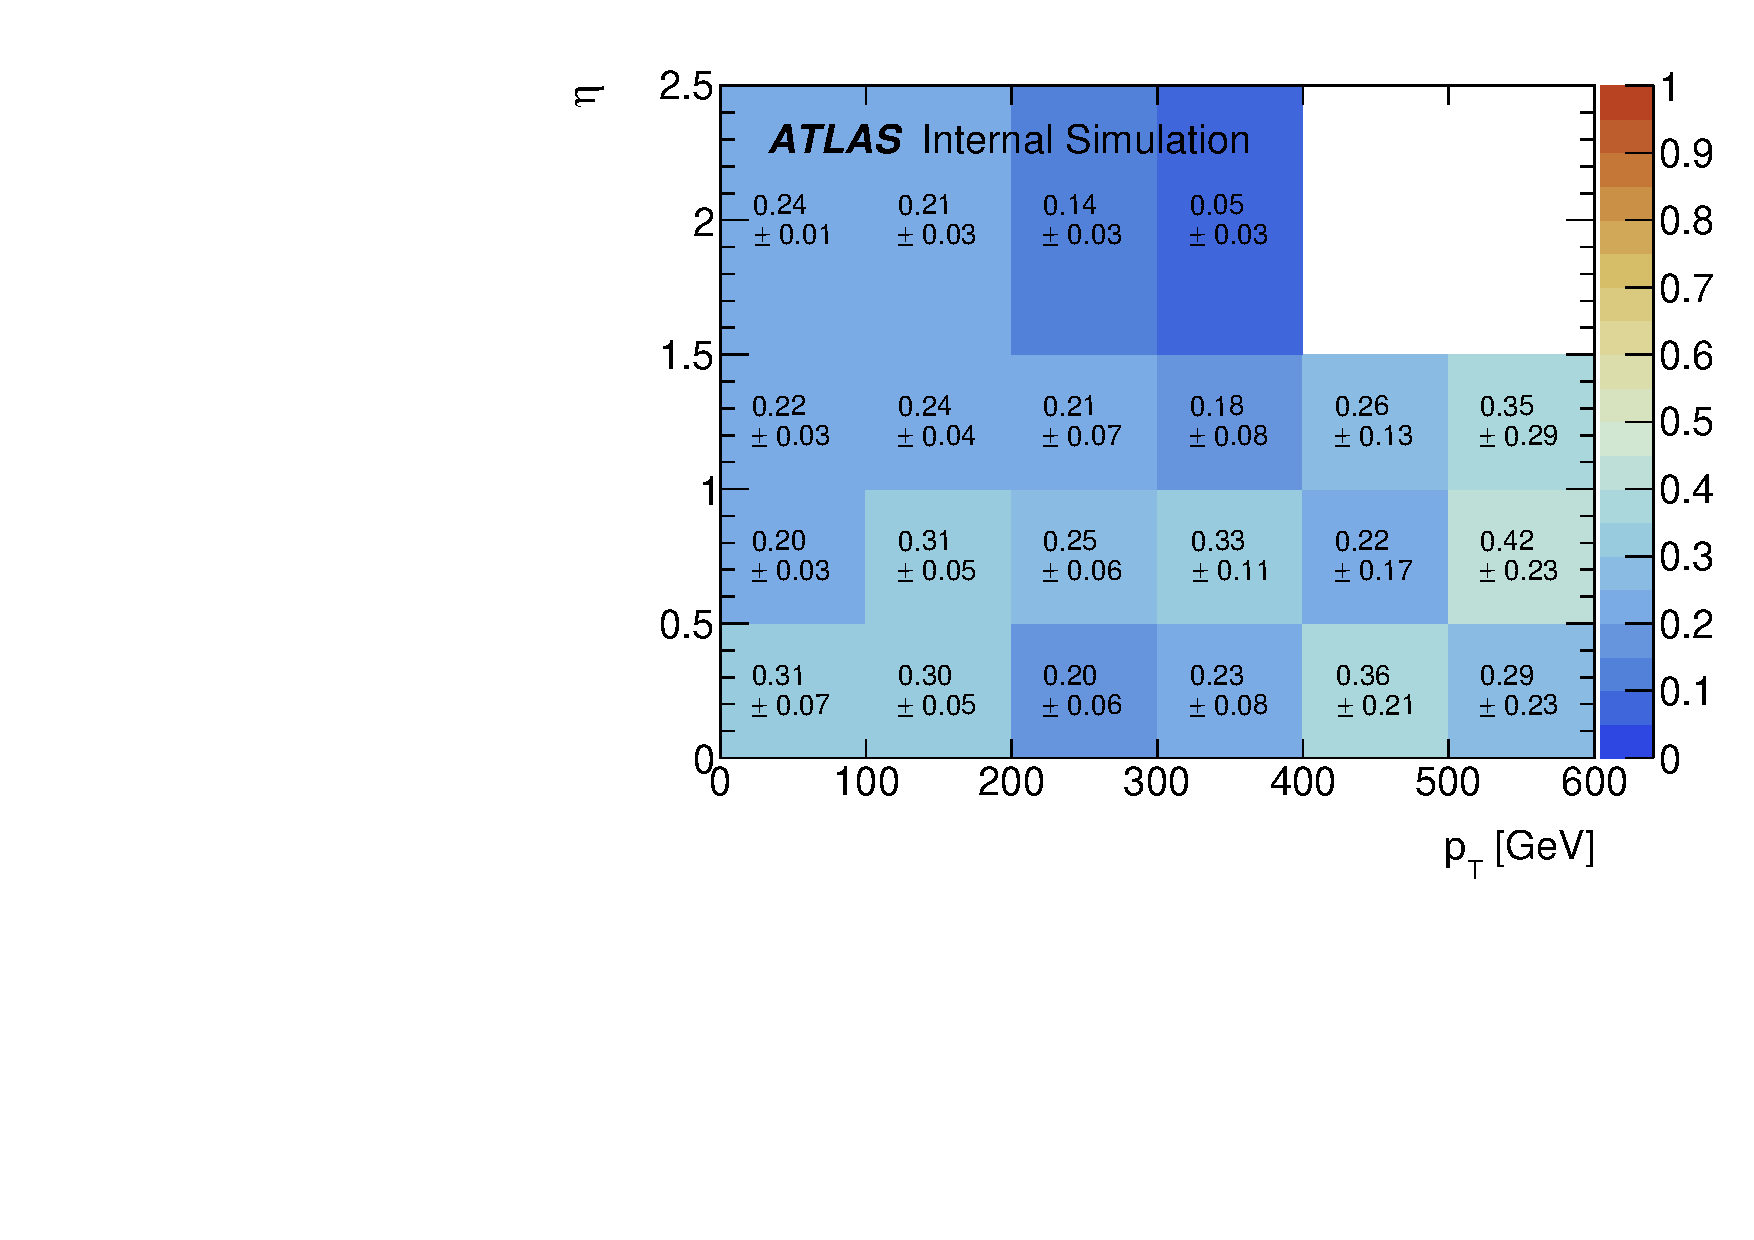
\includegraphics[width=0.50\textwidth]{figures/EfficiencyMap/eff_map_mumu_m500t100.pdf}}
    \subfloat[]{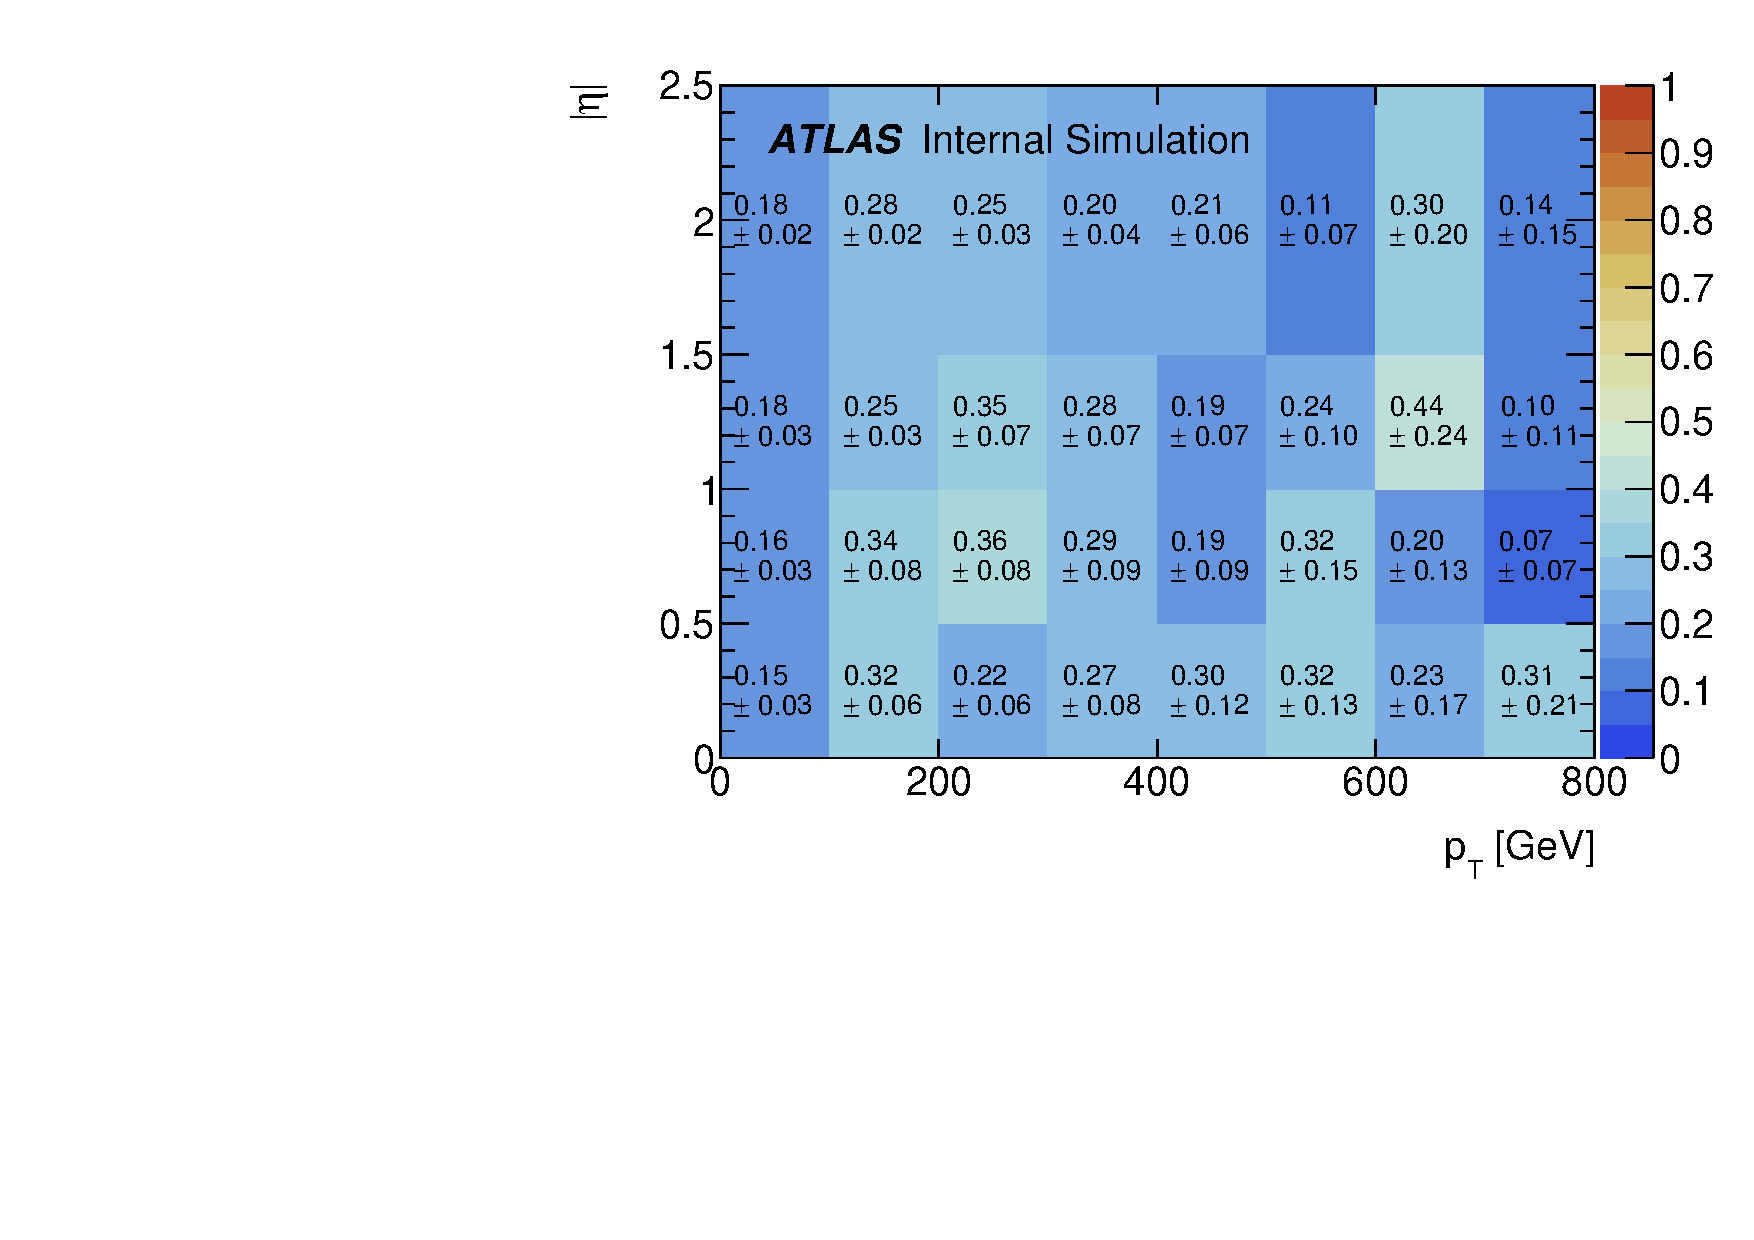
\includegraphics[width=0.50\textwidth]{figures/EfficiencyMap/eff_map_mumu_m1000t100.pdf}} \\
    \subfloat[]{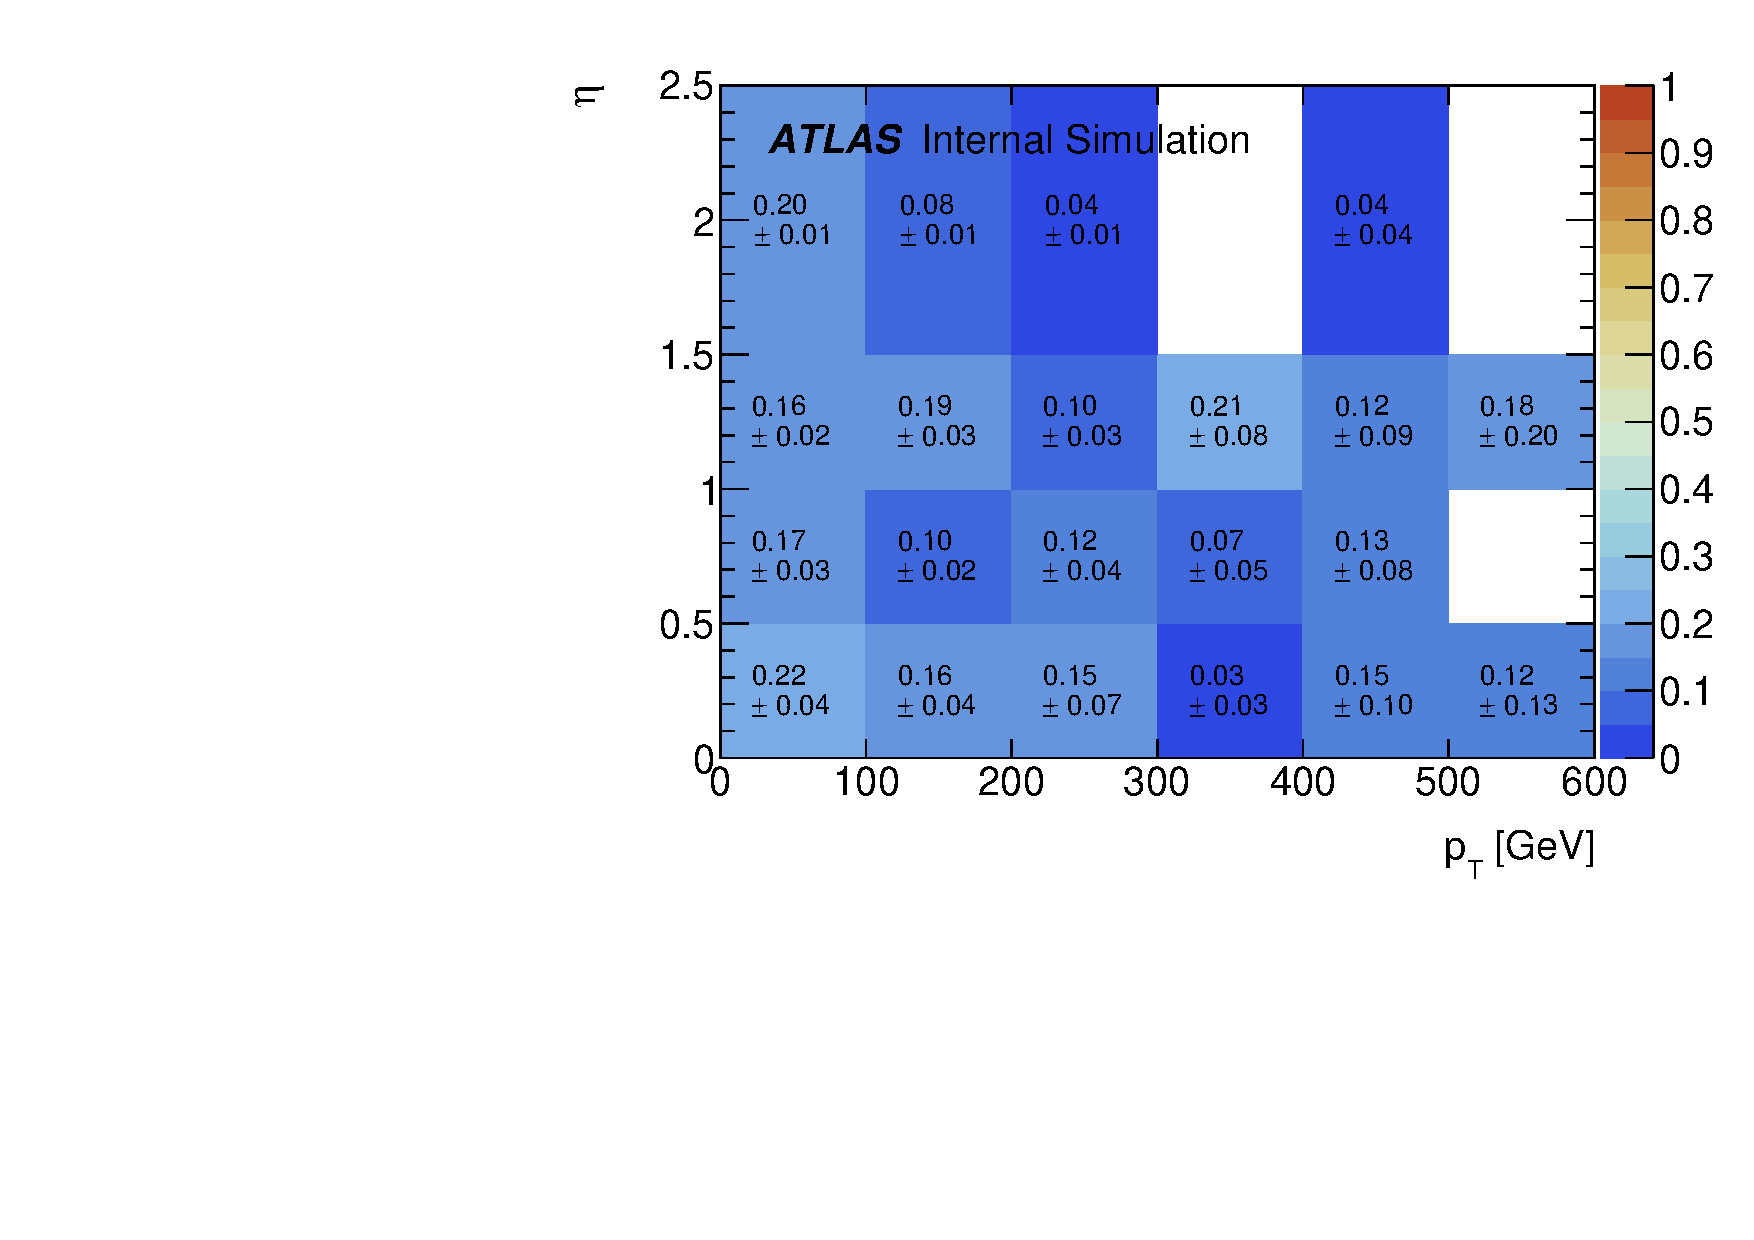
\includegraphics[width=0.50\textwidth]{figures/EfficiencyMap/eff_map_mumu_m500t500.pdf}}
    \subfloat[]{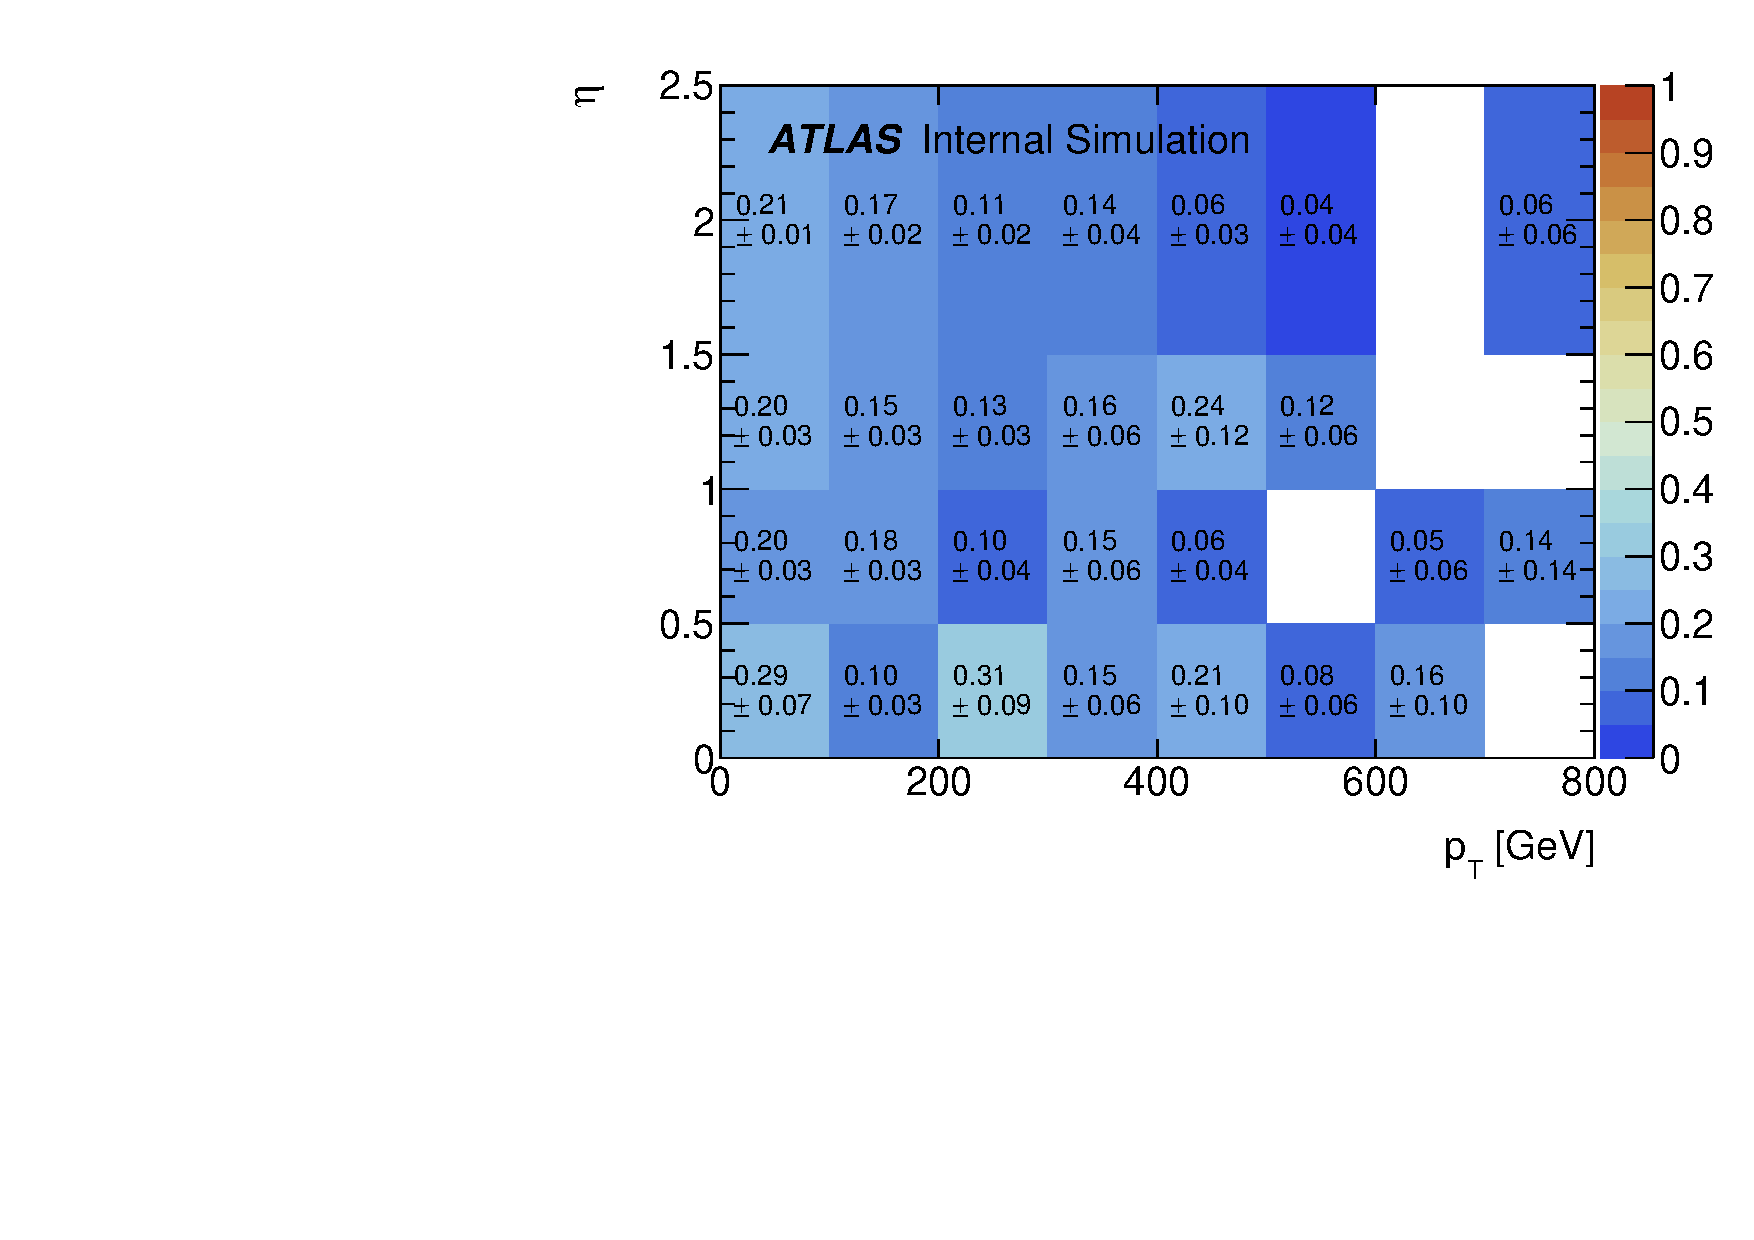
\includegraphics[width=0.50\textwidth]{figures/EfficiencyMap/eff_map_mumu_m1000t500.pdf}} \\
    \caption{Signal efficiency map of the signal MC sample with (a) $m=500$ and (b) $m=1000$ GeV for $c\tau=$ 100 mm. The corresponding efficiency map for $c\tau=$ 500 mm is shown in (c) and (d).}
    \label{fig:signal_eff_map}
\end{figure}




